\section{Experiments}
\label{sec:experiments}

The experimental evaluation of the proposed method are presented in this section. 
Section \ref{sec:exp_pre} introduces the details of custom dataset collected in the manner described in Section \ref{sec:proposed} and pre-processing.
Transfer learning of YOLOv8 using the custom dataset is covered in detail in Section \ref{sec:exp_transfer}.
Section \ref{sec:exp_results} describes the experimental results in detail.

\subsection{Custom dataset \& Pre-processing}
\label{sec:exp_pre}
A large-scale custom dataset of over 16 hours was collected. 
Videos from dashboard cameras were collected through real road driving for more than 16 hours, and total of more than 11K images were secured by setting the time interval $T$ to 5 seconds.
All secured images were manually annotated for the bounding box of the driving vehicle and the brake light status of each vehicle.
Total number of annotations are more than 30K.
We have split the collected dataset into train and test dataset, taking into consideration several factors during the split process.
These factors include data consistency, exclusion of duplicate or similar data, and data balance.
To ensure data diversity, driving scenarios include various environments such as daytime, nighttime, city, highway, and tunnel.
To address data balance, we took precautions to prevent any bias towards a single category.
The details of numbers of images and annotations in the train and test sets in each category of brake light status are given in Table \ref{tab:dataset}.




\begin{table}[h]
    \caption{Details of train and test datasets}
    \label{tab:dataset}
    % \resizebox{\textwidth*0.5}{!}{%
    \begin{tabular}{p{5cm} p{5cm} p{5cm}}
        % {lrr}
    \toprule
    \multicolumn{1}{c}{Number of}                          & \multicolumn{1}{c}{Train} & \multicolumn{1}{c}{Test} \\
    \midrule
    Images                              & \multicolumn{1}{r}{7,892}                     & \multicolumn{1}{r}{3,196}                    \\
    Annotations                         & \multicolumn{1}{r}{19,913}                    & \multicolumn{1}{r}{10,531}                   \\
    \multicolumn{1}{c}{Brake Light Off ($C_{1}=1.0$)} & \multicolumn{1}{r}{10,851}                    & \multicolumn{1}{r}{5,999}                    \\
    \multicolumn{1}{c}{Brake Light On ($C_{2}=1.0$)}  & \multicolumn{1}{r}{9,062}                     & \multicolumn{1}{r}{4,532}                   \\
    \bottomrule
    \end{tabular}%
    % }
\end{table}



For our custom dataset to be trainable with YOLOv8 and get results showing robust performance, several pre-processing is required.
The first essential processes are image resizing and normalization.
Since the shape of the input image must always be the same, the width and height of all images were resized to $I_{w}$ and $I_{h}$. In this study, both $I_{w}$ and $I_{h}$ were defined as $640$. 
In the case of image normalization, min-max normalization was applied to all pixel values as follows:

\begin{equation}
    x_{norm} = \frac{x - x_{min}}{x_{max} - x_{min}}
\end{equation}
where $x$ and $x_{norm}$ are origin and normalized pixel value, respectively and $x_{max}$ and $x_{min}$ are the maximum and minimum pixel value of the image, respectively.
As usual, in this study, $x_{max}$ and $x_{min}$ were defined as $255.0$ and $0.0$.
In addition, various data augmentation techniques were applied for robust inference performance.
Random horizontal flip and crop image were performed to create image that was different from the collected images and could actually exist.
For robust detection even in occlusion, the random black-box cutout is also applied.
Lastly, in terms of securing robustness for various cameras, the quality of input images was degraded in various ways.

\begin{figure}[b!]%

    \subfloat{{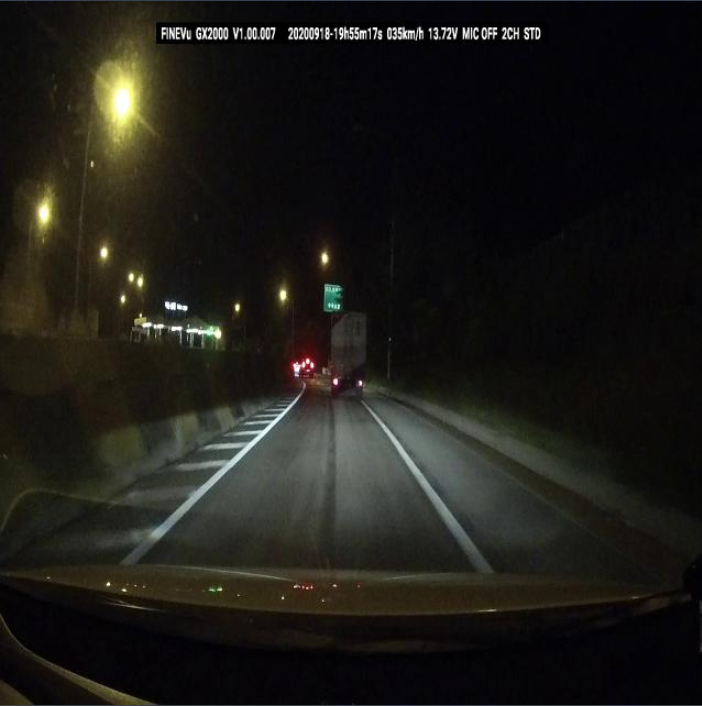
\includegraphics[height=4.5cm]{fig/image20.png} }}%
    \subfloat{{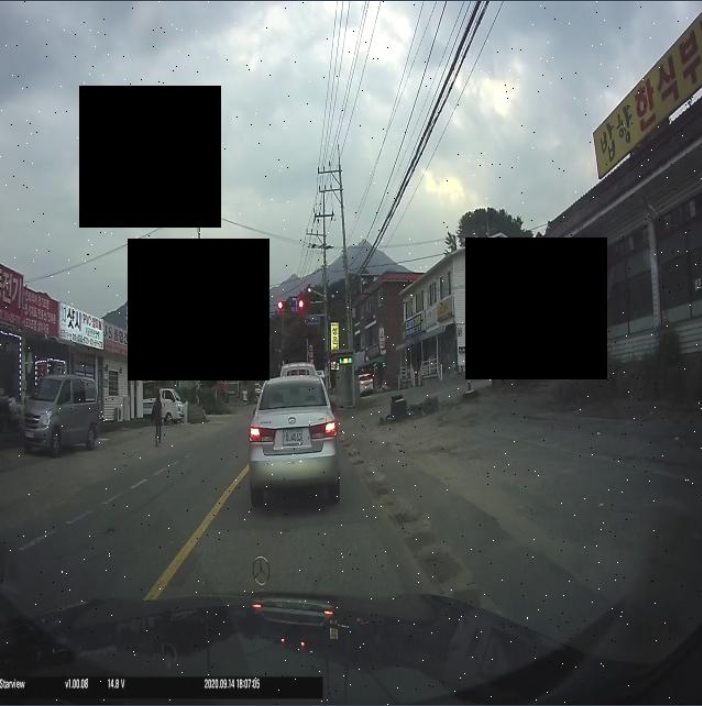
\includegraphics[height=4.5cm]{fig/image21.png} }}%
    \subfloat{{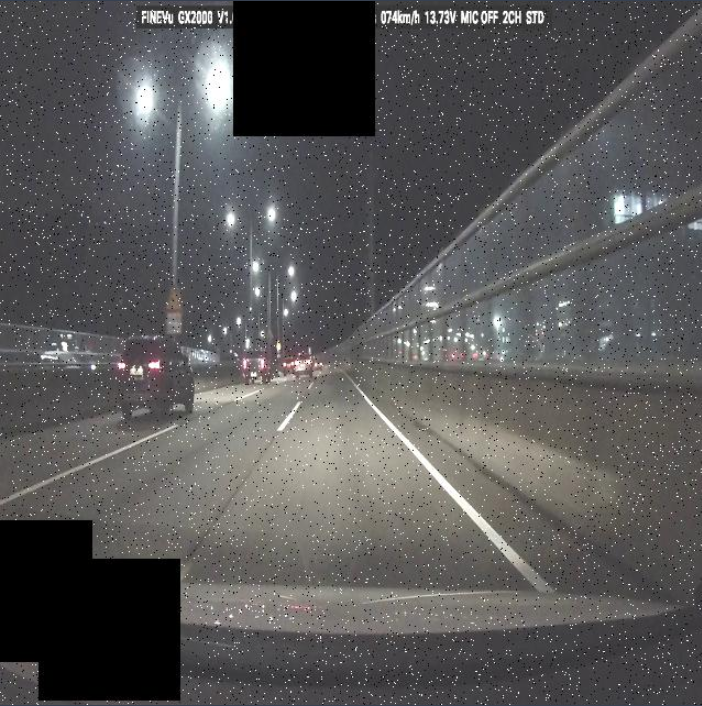
\includegraphics[height=4.5cm]{fig/image22.png} }}%
    \hfill
    \subfloat{{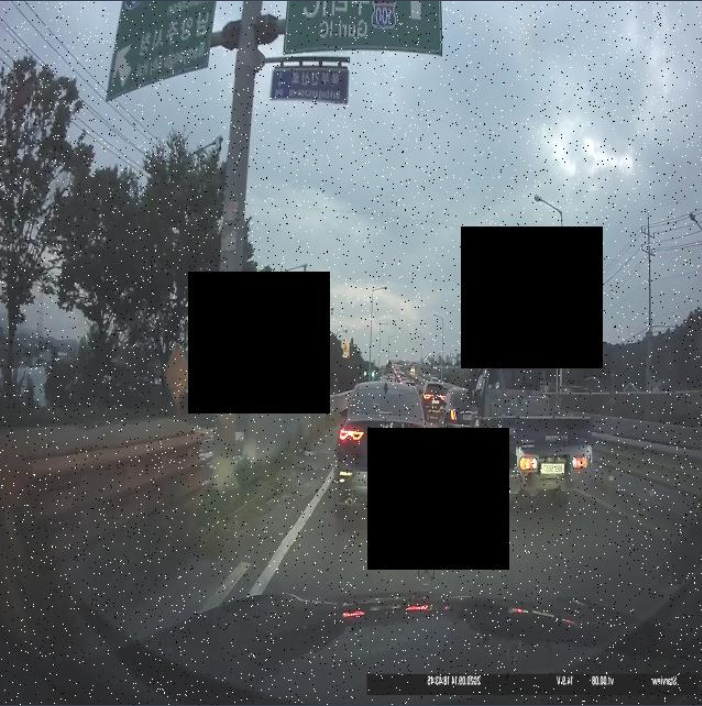
\includegraphics[height=4.5cm]{fig/image23.png} }}%
    \subfloat{{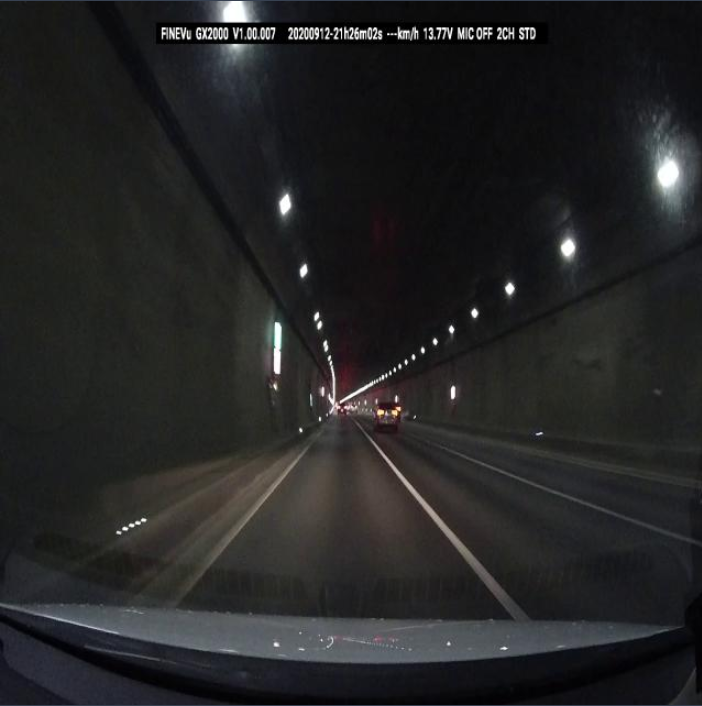
\includegraphics[height=4.5cm]{fig/image24.png} }}%
    \subfloat{{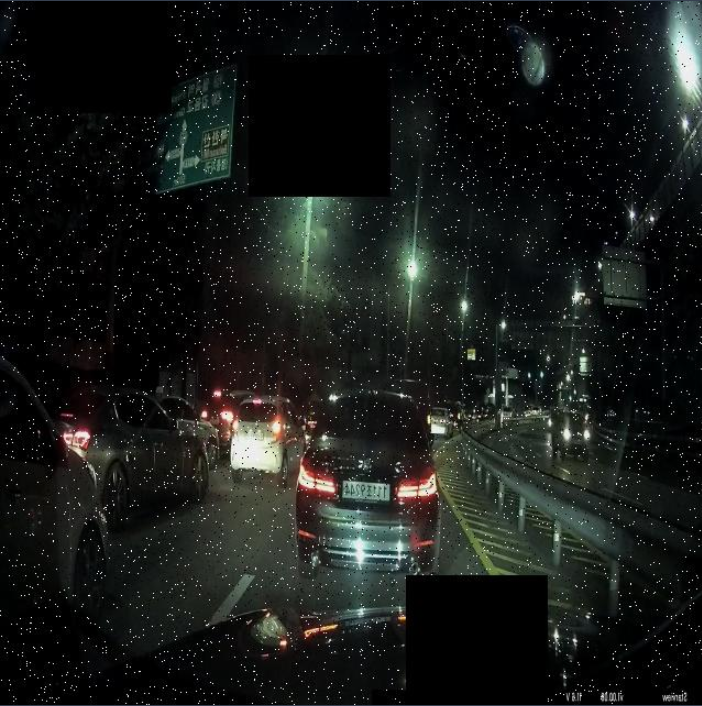
\includegraphics[height=4.5cm]{fig/image25.png} }}%

\caption{Pre-processed input images of custom dataset}
\label{fig:custom_dataset}%
\end{figure}

As mentioned in Section \ref{sec:method_dataset}, the dashboard cameras used for image acquisition includes various post-processing methods to acquire high-quality images.
Therefore, brightness change, blur, and noise injection methods were randomly applied to ensure robust performance of the trained network even in general cameras.
Examples of pre-processed image are shown in Figure \ref{fig:custom_dataset}.
All pre-processing processes utilized Roboflow \cite{roboflow}, which is a comprehensive platform for computer vision and image processing task, and pre-processed train dataset is publicly available \cite{brake-light-detection_dataset}.

\begin{table}[h]
    \caption{Official deplyed models of YOLOv8}
    \label{tab:yolov8}
    % \resizebox{\textwidth}{!}{%
    \begin{tabular}{lcc}
    \toprule
    \multicolumn{1}{c}{Model}   & \# params (M) & FLOPs (B) \\
    \midrule
    YOLOv8n & 3.2        & 8.7       \\
    YOLOv8s & 11.2       & 28.6      \\
    YOLOv8m & 25.9       & 78.9      \\
    YOLOv8l & 43.7       & 165.2     \\
    YOLOv8x & 68.2       & 257.8     \\
    \bottomrule
    \multicolumn{3}{l}{\textit{Note:} All values in the table correspond}\\
    \multicolumn{3}{l}{\qquad \; to an input image size of 640x640.}
    \end{tabular}%
    % }
\end{table}

\subsection{Transfer learning}
\label{sec:exp_transfer}
YOLOv8 \cite{YOLOv8} has officially deployed a total of five models of different sizes, from the smallest model, YOLOv8n, to the largest model, YOLOv8x as described in Table \ref{tab:yolov8}.
In this study, the objective is to develop a detection network that can perform real-time inference in a driving vehicle while achieving accurate detection. 
To achieve this, we conducted transfer learning on all models provided by YOLOv8 and derived optimal trade-off performance by experimenting with detection performance and inference speed.

The hyperparameters required for training were applied equally to all models, and the details are described in this paragraph.
20\% of train dataset had been randomly split into the validation dataset.
The initial value of each model parameter used pre-trained parameters officially provided by YOLOv8 \cite{YOLOv8}.
Number of iterations and patience were defined as $300$ and $20$, respectively.
During the 300 iterations, if there is no observable improvement among the latest 20 iterations, the learning was terminated to reduce the consumption of time and resources.
We used a stochastic gradient descent (SGD) optimizer with $0.01$ learning rate.
The optimizer incorporated both momentum and Nesterov Accelerated Gradient (NAG) techniques \cite{sutskever2013importance} and the momentum coefficient was defined as $0.937$.
The weighting factors assigned to the three loss functions used in training, binary cross-entropy, CIoU, and DFL, are $0.5$, $7.5$, and $1.5$, respectively.


\begin{figure}[t]%

    \subfloat{{\includegraphics[height=1.9cm]{fig/Capture/0_highway.jpg} }}%
    \subfloat{{\includegraphics[height=1.9cm]{fig/Capture/0_city.jpg} }}%
    \subfloat{{\includegraphics[height=1.9cm]{fig/Capture/0_tunnel.jpg} }}%
    \subfloat{{\includegraphics[height=1.9cm]{fig/Capture/0_night.jpg} }}%
    \hfill
    \subfloat{{\includegraphics[height=1.9cm]{fig/Capture/0_motor.jpg} }}%
    \subfloat{{\includegraphics[height=1.9cm]{fig/Capture/0_bus.jpg} }}%
    \subfloat{{\includegraphics[height=1.9cm]{fig/Capture/0_truck.jpg} }}%
    \subfloat{{\includegraphics[height=1.9cm]{fig/Capture/0_special_1.jpg} }}%

\caption{Images of driving vehicle and brake light status detection results by proposed networks. Images in the first row depict the detection results in various road environments. From left to right, the depicted environments are highway, city, tunnel, and nighttime. Images in the second row depict the detection results of various vehicle types. From left to right, the depicted vehicle types include motorcycle, bus, trucks, and special vehicle.}
\label{fig:detection}%
\end{figure}




\subsection{Results}
\label{sec:exp_results}
In this section, the qualitative and quantitative evaluation results of the trained detection models were described.
Qualitative analysis confirmed that the trained detection models accurately detect the bounding boxes of driving vehicles and classify their brake light status as either the brake on or off in various road environments. 
The models exhibited robust performance in highway, city, tunnel, and nighttime driving scenarios, demonstrating excellent detection results not only conventional passenger cars but also motorcycles, buses, trucks and special vehicles.
The qualitative detection results are shown in Figure \ref{fig:detection}.


The driving vehicle and brake light status detection performance of each model that has completed transfer learning is evaluated by calculating the mean average precision (mAP) in the testset.
We calculated a total of two mAP: mAP50 and mAP50-95.
mAP50 represents the mAP at an intersection over union (IoU) threshold of $0.5$. Here, the IoU threshold indicates the ratio of the overlapping area between the predicted bounding boxes and the ground truth labels.
On the other hand, mAP50-95 represents the average precision over a range of IoU thresholds from $0.5$ to $0.95$ with a step size $0.05$. 
Both of mAP are commonly used as a comprehensive measure to assess the overall performance of object detection models.

\begin{figure}[t]%

    \subfloat[\centering mAP50 on the entire testset]{{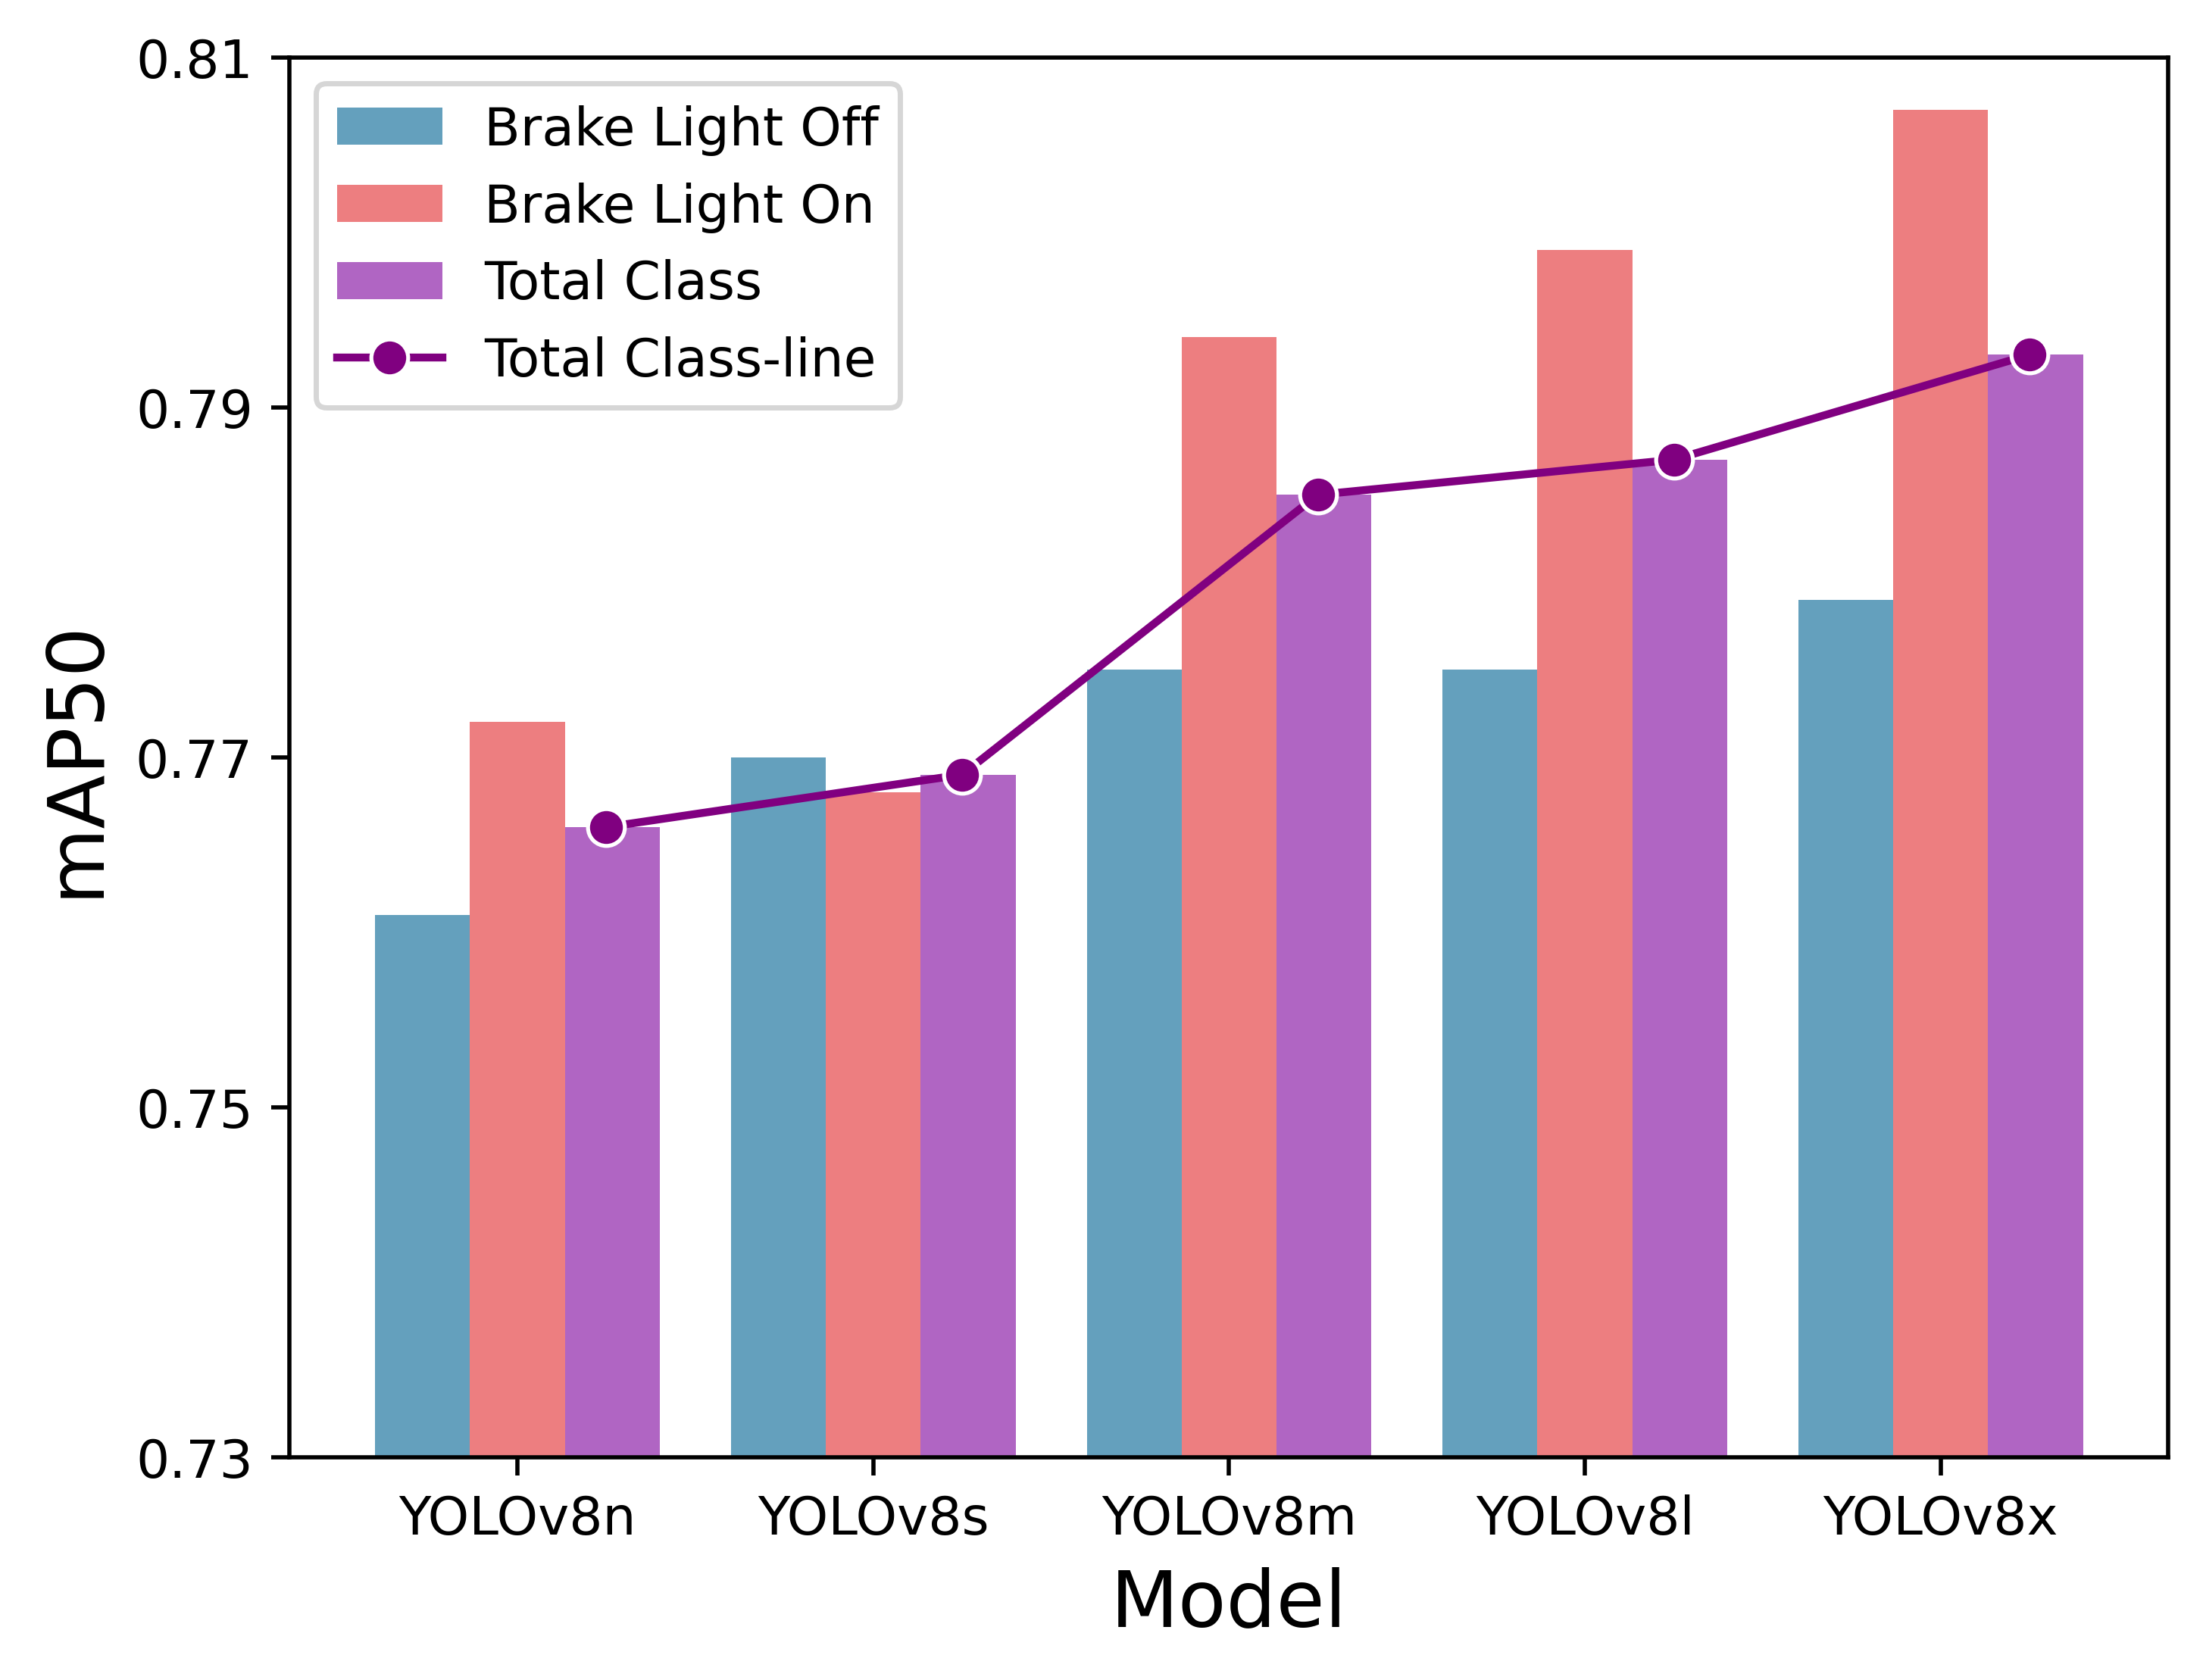
\includegraphics[height=5cm]{fig/bar_map50.png} }}%
    \subfloat[\centering mAP50-95 on the entire testset]{{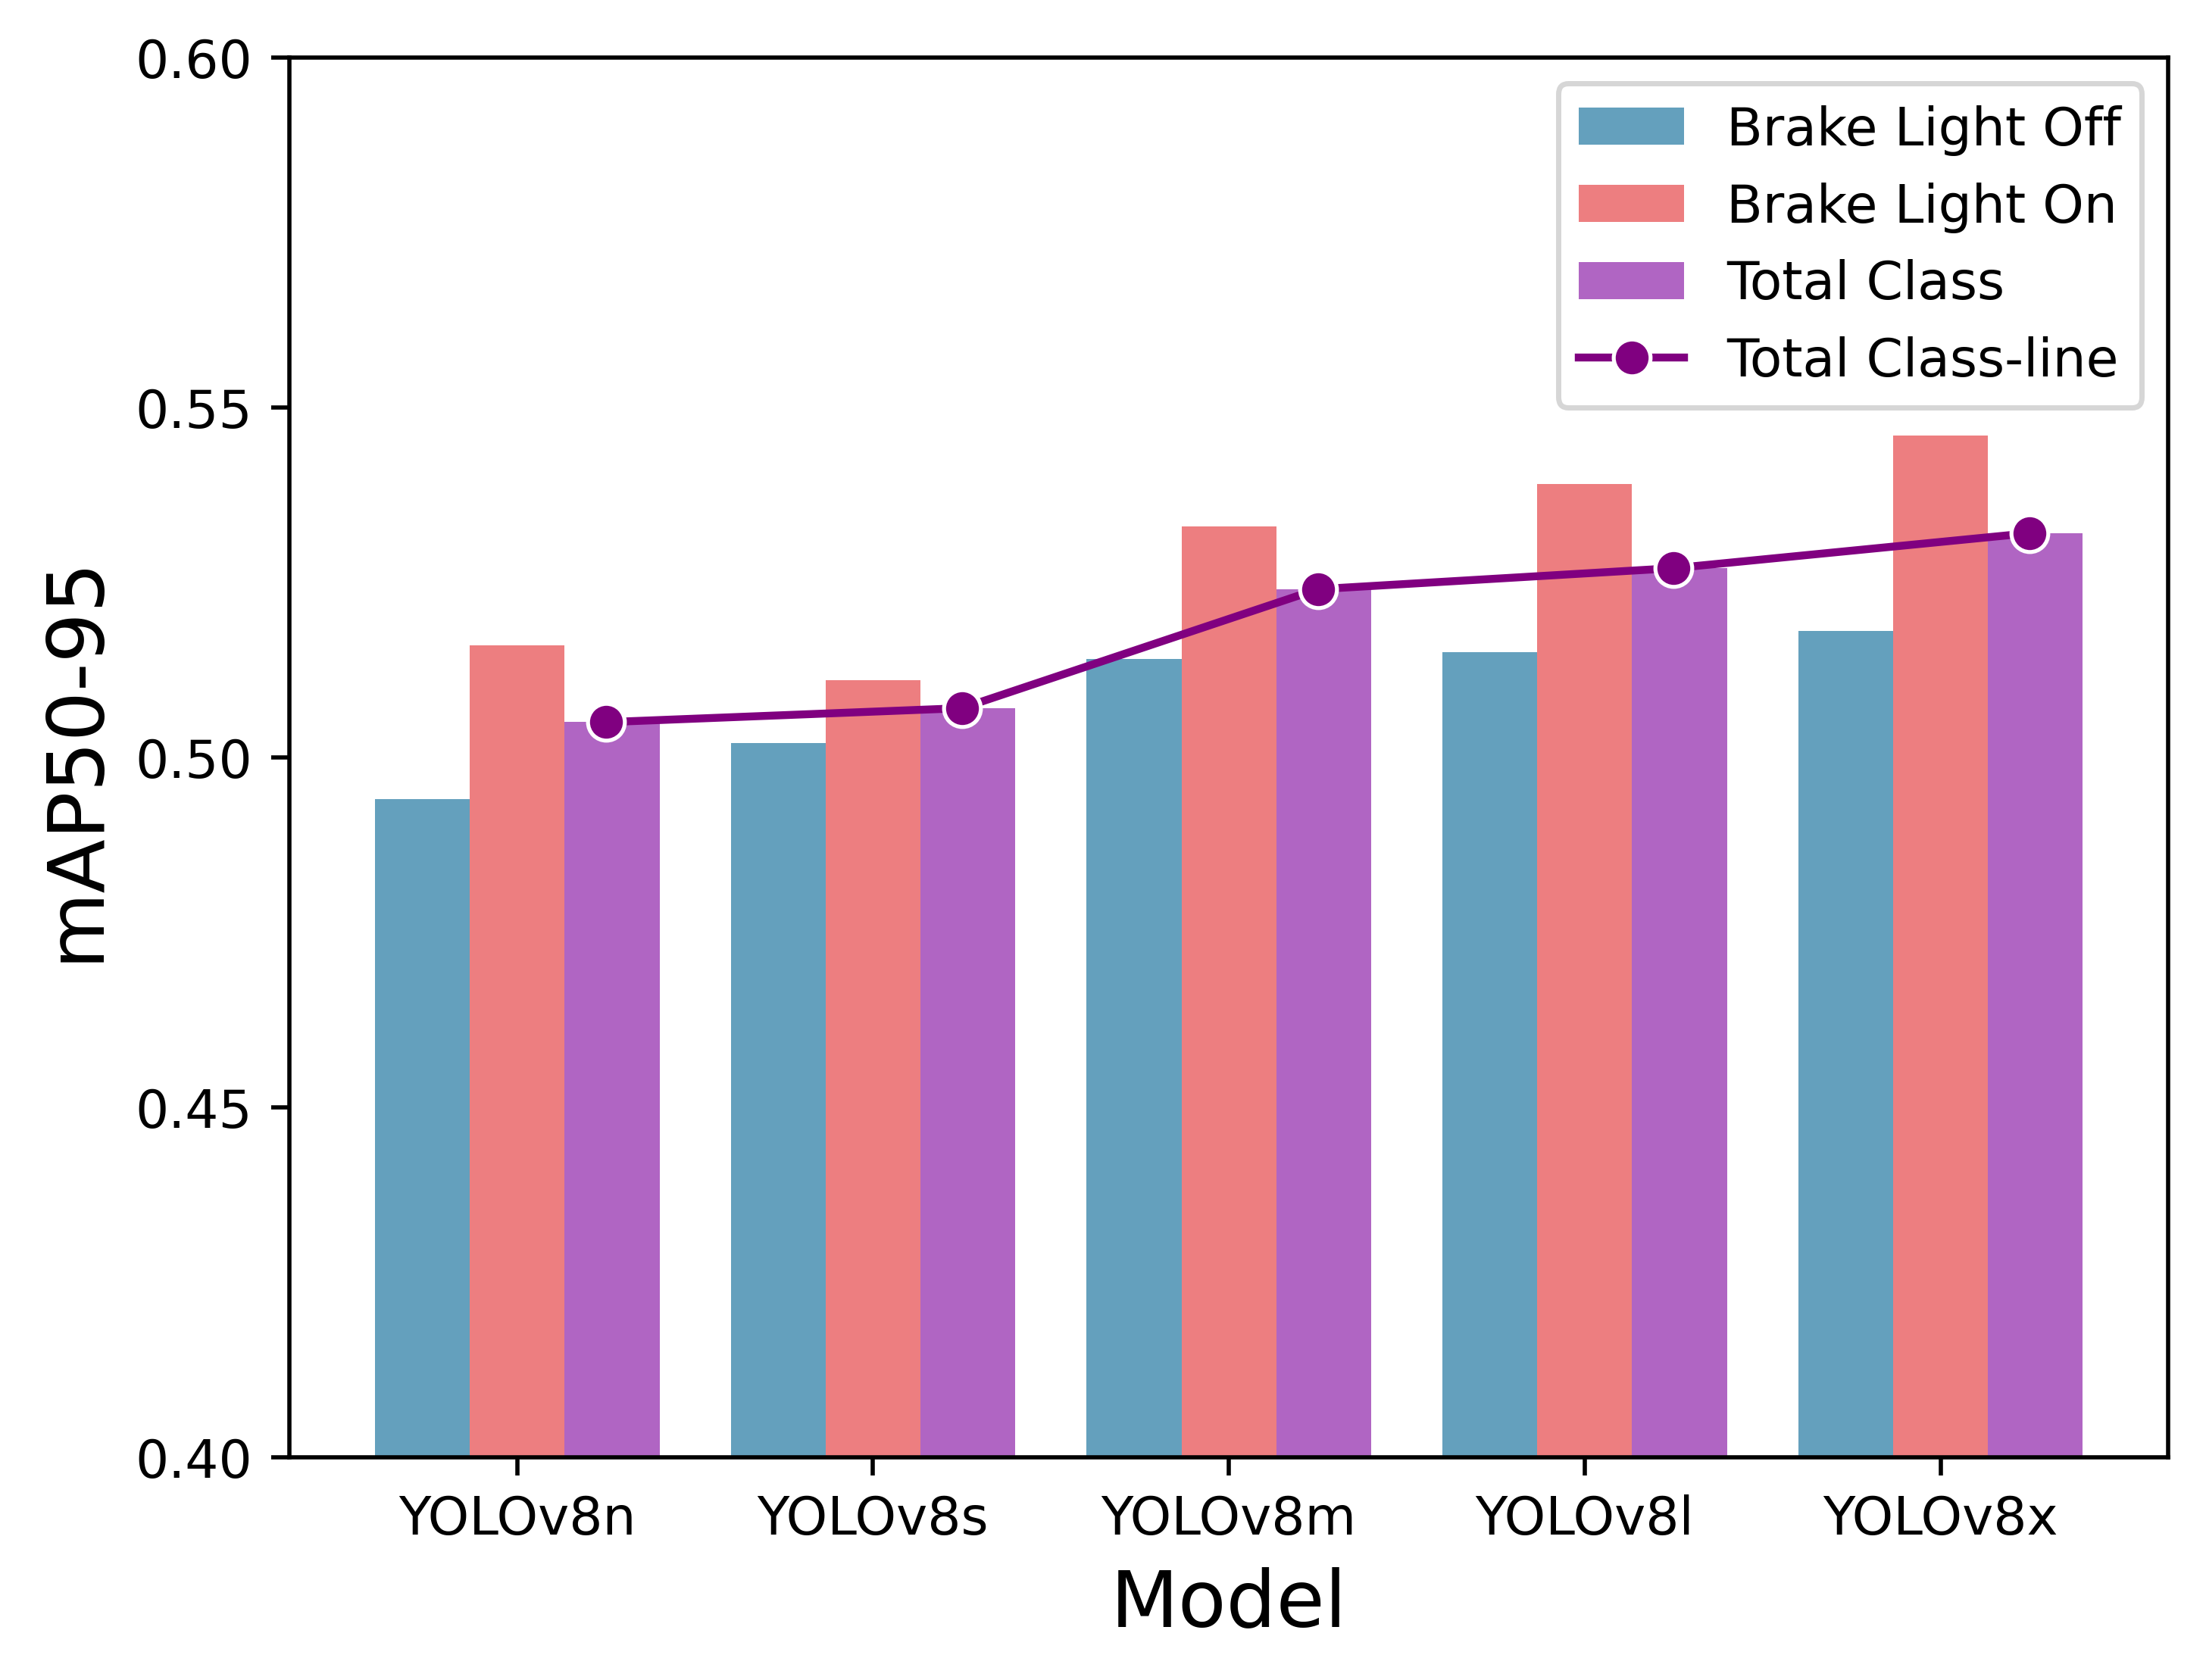
\includegraphics[height=5cm]{fig/bar_map50-95.png} }}%

\caption{Detection performance on the entire testset. The y-axis represents the detection accuracy, and the x-axis lists the YOLOv8 models, with larger models positioned towards the right. Each model is depicted with three bars, showcasing the detection performance for brake light off class, brake light on class, and total class, respectively. Single line plot highlights the difference in detection performance by models for total class.}
\label{fig:test_results}%
\end{figure}

\begin{table}[!h]
    \caption{Results of the entire testset}
    \label{tab:total}
    % \resizebox{\textwidth}{!}{%
    % \begin{tabular}{>{\raggedright}p{2.5cm} >{\raggedright}p{2.5cm} >{\centering}p{2.5cm} >{\centering\arraybackslash}p{2.5cm}}
    \begin{tabular}{llrr}
    \toprule
    \multicolumn{1}{c}{Model} & \multicolumn{1}{c}{Class} & \multicolumn{1}{c}{mAP50} & \multicolumn{1}{c}{mAP50-95} \\
    \midrule
    \multirow{3}{*}{YOLOv8n}  & Brake Light Off           & 0.761                     & 0.494                          \\
                              & Brake Light On            & 0.772                     & 0.516                        \\
                              & \multicolumn{1}{r}{Total} & 0.766                     & 0.505                        \\
    \midrule
    \multirow{3}{*}{YOLOv8s}  & Brake Light Off           & 0.770                     & 0.502                        \\
                              & Brake Light On            & 0.768                     & 0.511                        \\
                              & \multicolumn{1}{r}{Total} & 0.769                     & 0.507                        \\
    \midrule
    \multirow{3}{*}{YOLOv8m}  & Brake Light Off           & 0.775                     & 0.514                         \\
                              & Brake Light On            & 0.794                     & 0.533                        \\
                              & \multicolumn{1}{r}{Total} & 0.785                     & 0.524                        \\
    \midrule
    \multirow{3}{*}{YOLOv8l}  & Brake Light Off           & 0.775                     & 0.515                         \\
                              & Brake Light On            & 0.799                     & 0.539                        \\
                              & \multicolumn{1}{r}{Total} & 0.787                     & 0.527                      \\
    \midrule
    \multirow{3}{*}{YOLOv8x}  & Brake Light Off           & 0.779                     & 0.518                         \\
                              & Brake Light On            & 0.807                     & 0.546                        \\
                              & \multicolumn{1}{r}{Total} & 0.793                     & 0.532                      \\
    \bottomrule
    \end{tabular}%
    % }
\end{table}

Figure \ref{fig:test_results} presents the detection performance of each trained model.
Figure \ref{fig:test_results}-(a) and (b) are the plot for mAP50 and mAP50-95, respectively.
Each individual classes, brake light off and on, detection performance are shown in blue and red bars, respectively.
The detection performance for all classes is shown in purple bar with the purple line plot to effectively show the trend of performance differences by model.
Although mAP50 and mAP50-95 differ in scale, they show almost similar overall trends.
As expected, detection performance for all classes increases as the size of the model increases.
The performance increase of the YOLOv8s model tends to be slightly lacking, which is analyzed to be due to the lack of brake light on class detection performance.
In fact, comparing the mAP50 for each class, the brake light on class detection performance of all models except YOLOv8s is higher than the brake light off class.
As a result, we achieved mAP50 from $0.766$ to $0.793$ and mAP50-95 from $0.505$ to $0.532$.
Considering the recent benchmarking performance of MS-COCO \cite{lin2014microsoft}, which is one of the most prominent object detection datasets today, with mAP50 of $71.9$ to $77.0$ and mAP50-95 of $57.7$ to $58.8$ \cite{coco_benchmark, zou2023object}, our proposed methodology can be regarded as yielding significant results. Detailed detection performance for each model and class is described in Table \ref{tab:total}.

\begin{table}[h]
    \caption{Details of test dataset}
    \label{tab:test_dataset}
    % \resizebox{\textwidth*0.5}{!}{%
    \begin{tabular}{p{5cm} p{5cm} p{5cm}}
        % {lrr}
    \toprule
    \multicolumn{1}{c}{Number of}                          & \multicolumn{1}{c}{Day} & \multicolumn{1}{c}{Night} \\
    \midrule
    Images                              & \multicolumn{1}{r}{1,467}                     & \multicolumn{1}{r}{1,729}                    \\
    Annotations                         & \multicolumn{1}{r}{4,911}                    & \multicolumn{1}{r}{5,620}                   \\
    \multicolumn{1}{c}{Brake Light Off ($C_{1}=1.0$)} & \multicolumn{1}{r}{3,563}                    & \multicolumn{1}{r}{2,436}                    \\
    \multicolumn{1}{c}{Brake Light On ($C_{2}=1.0$)}  & \multicolumn{1}{r}{1,348}                     & \multicolumn{1}{r}{3,184}                   \\
    \bottomrule
    \end{tabular}%
    % }
\end{table}

In Figure \ref{fig:test_results}, it was confirmed that brake light on detection performance was better than brake light off, but the two classes should be distinguished only by the brightness of the brake light, not the difference in the shape or form of the vehicle. 
Therefore, it is possible to establish a hypothesis that the ambient illumination can affect the detection performance, and to verify it, it is necessary to compare the detection performance in environments with different ambient illumination.
Then, we split the test dataset into two types according to the ambient light level. 
Images taken during daytime with high ambient illumination were named Day. 
Conversely, images taken at night or in tunnels with low ambient illumination were named Night, and the number of images and annotations are described in Table \ref{tab:test_dataset}.

\begin{figure}[t]%

    \subfloat[mAP50 on the Day testset]{{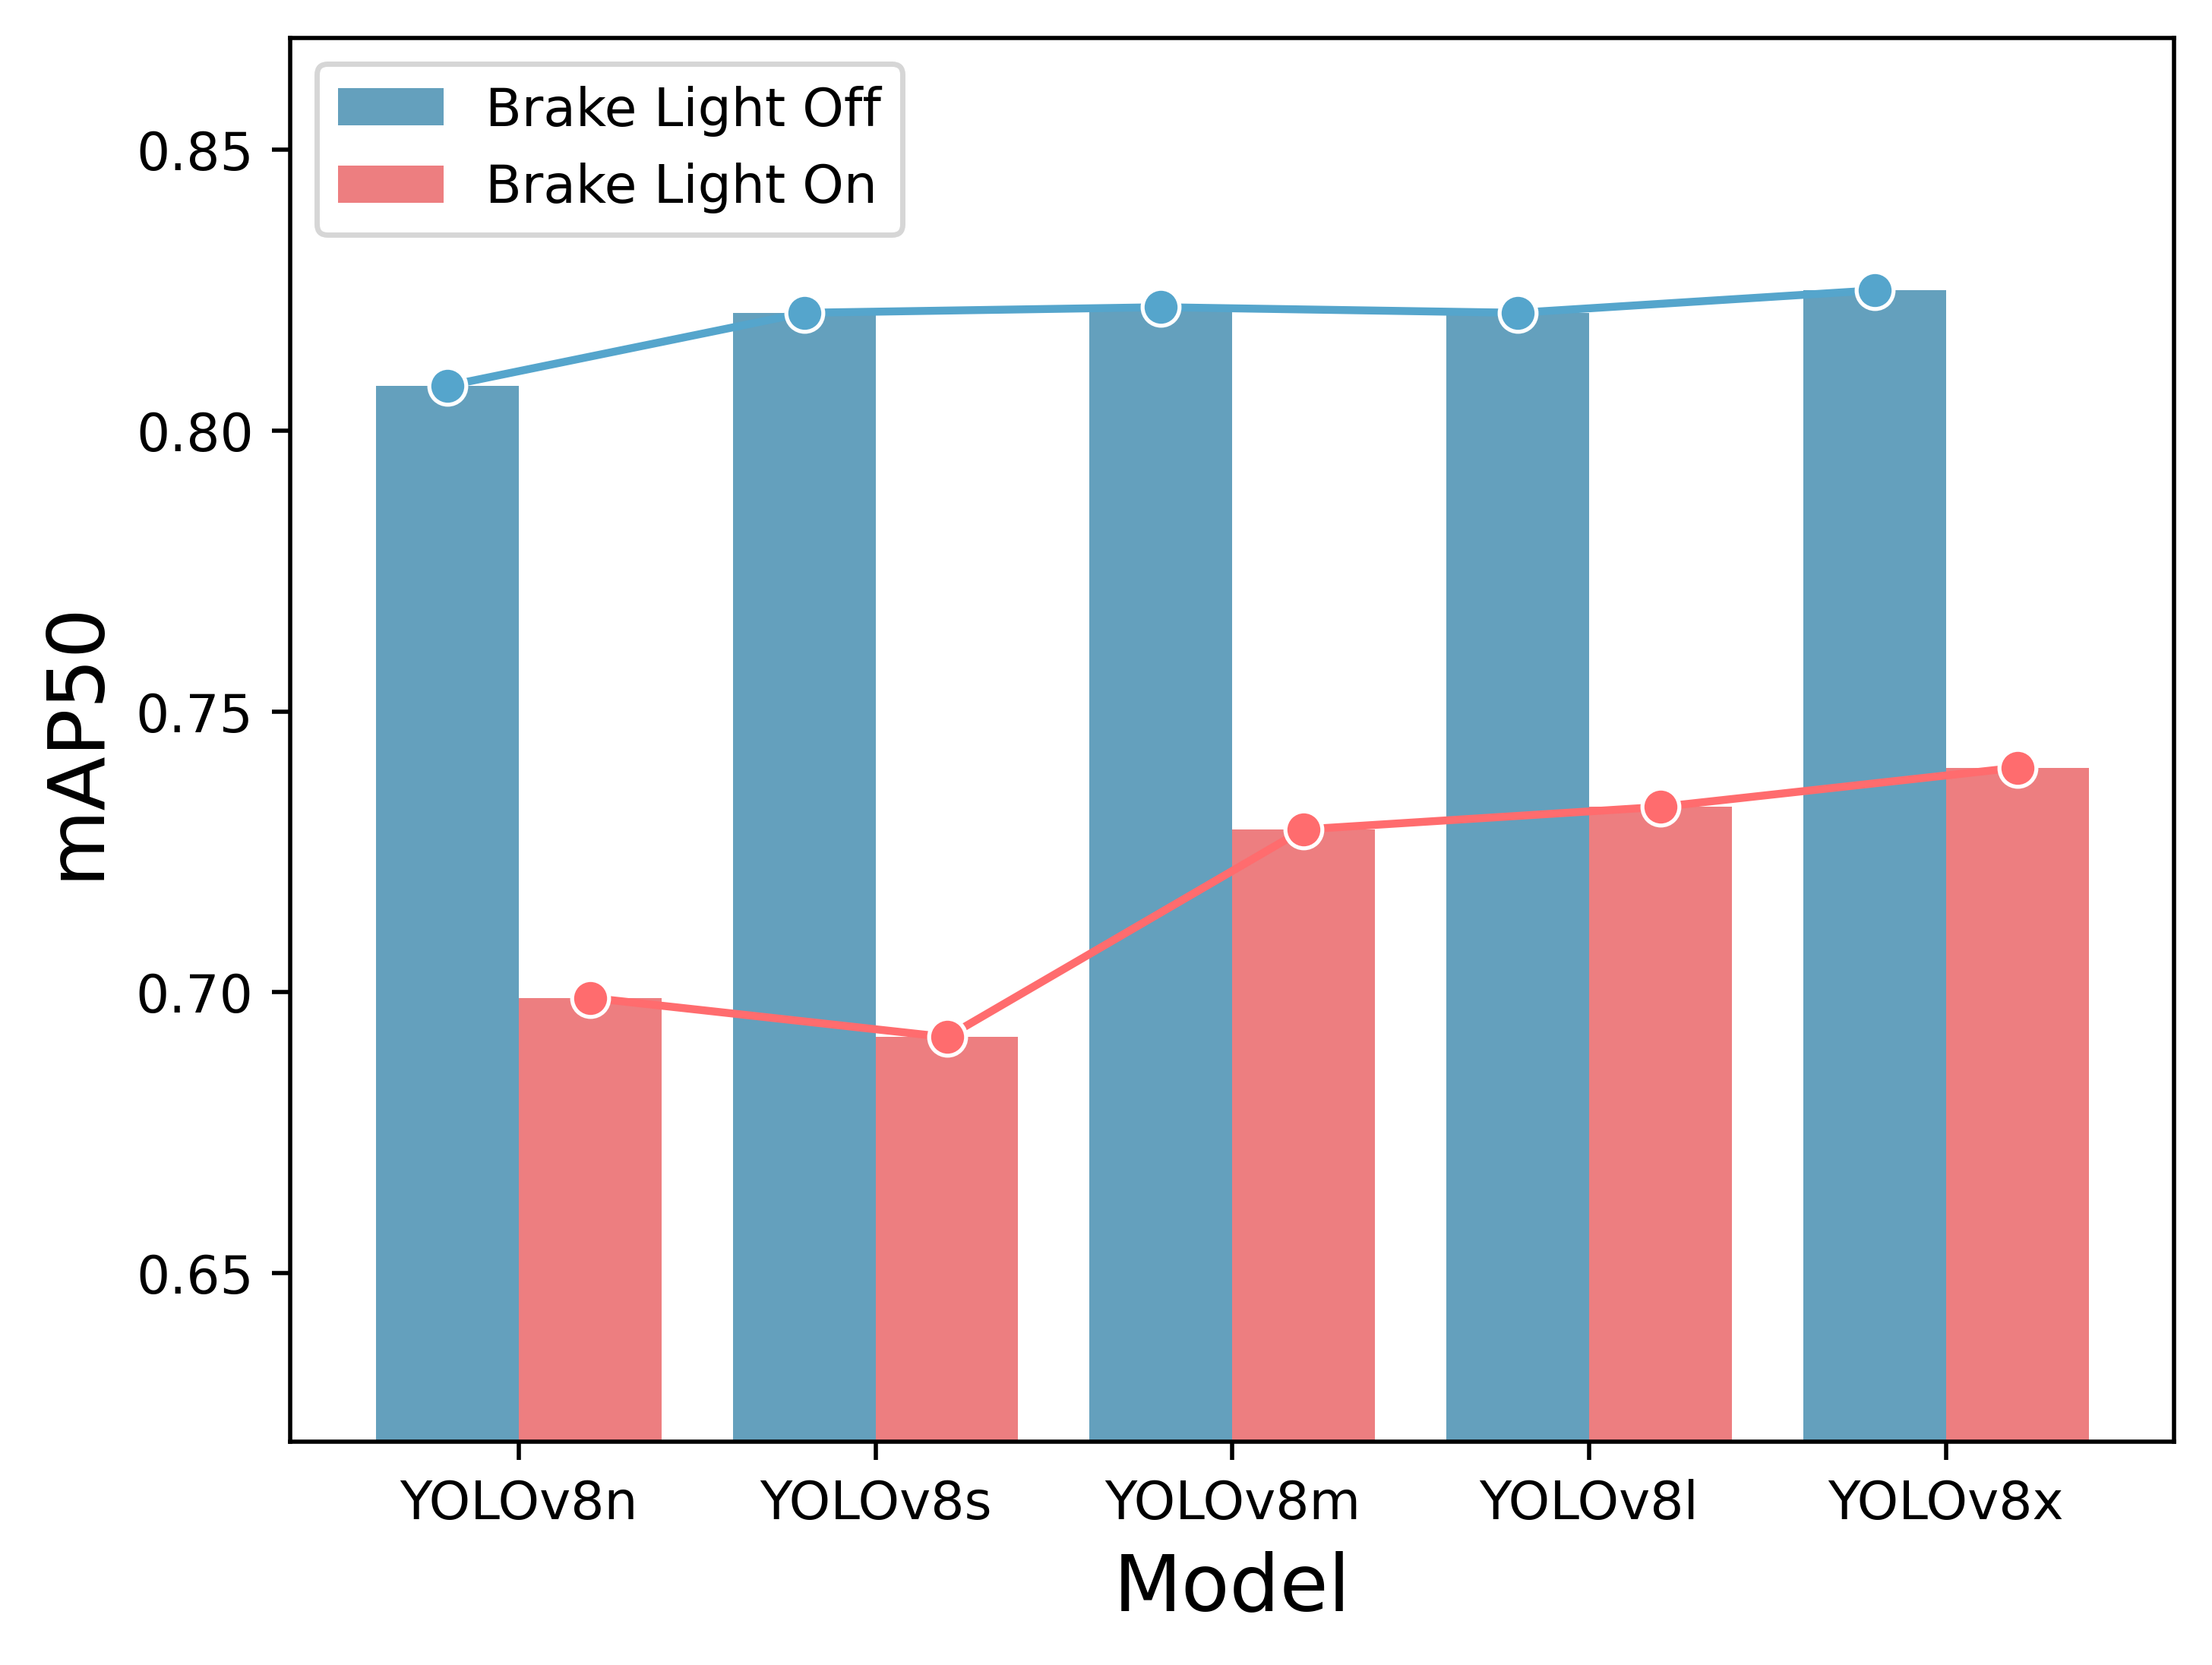
\includegraphics[height=5cm]{fig/bar_day_map50.png} }}%
    \subfloat[mAP50 on the Night testset]{{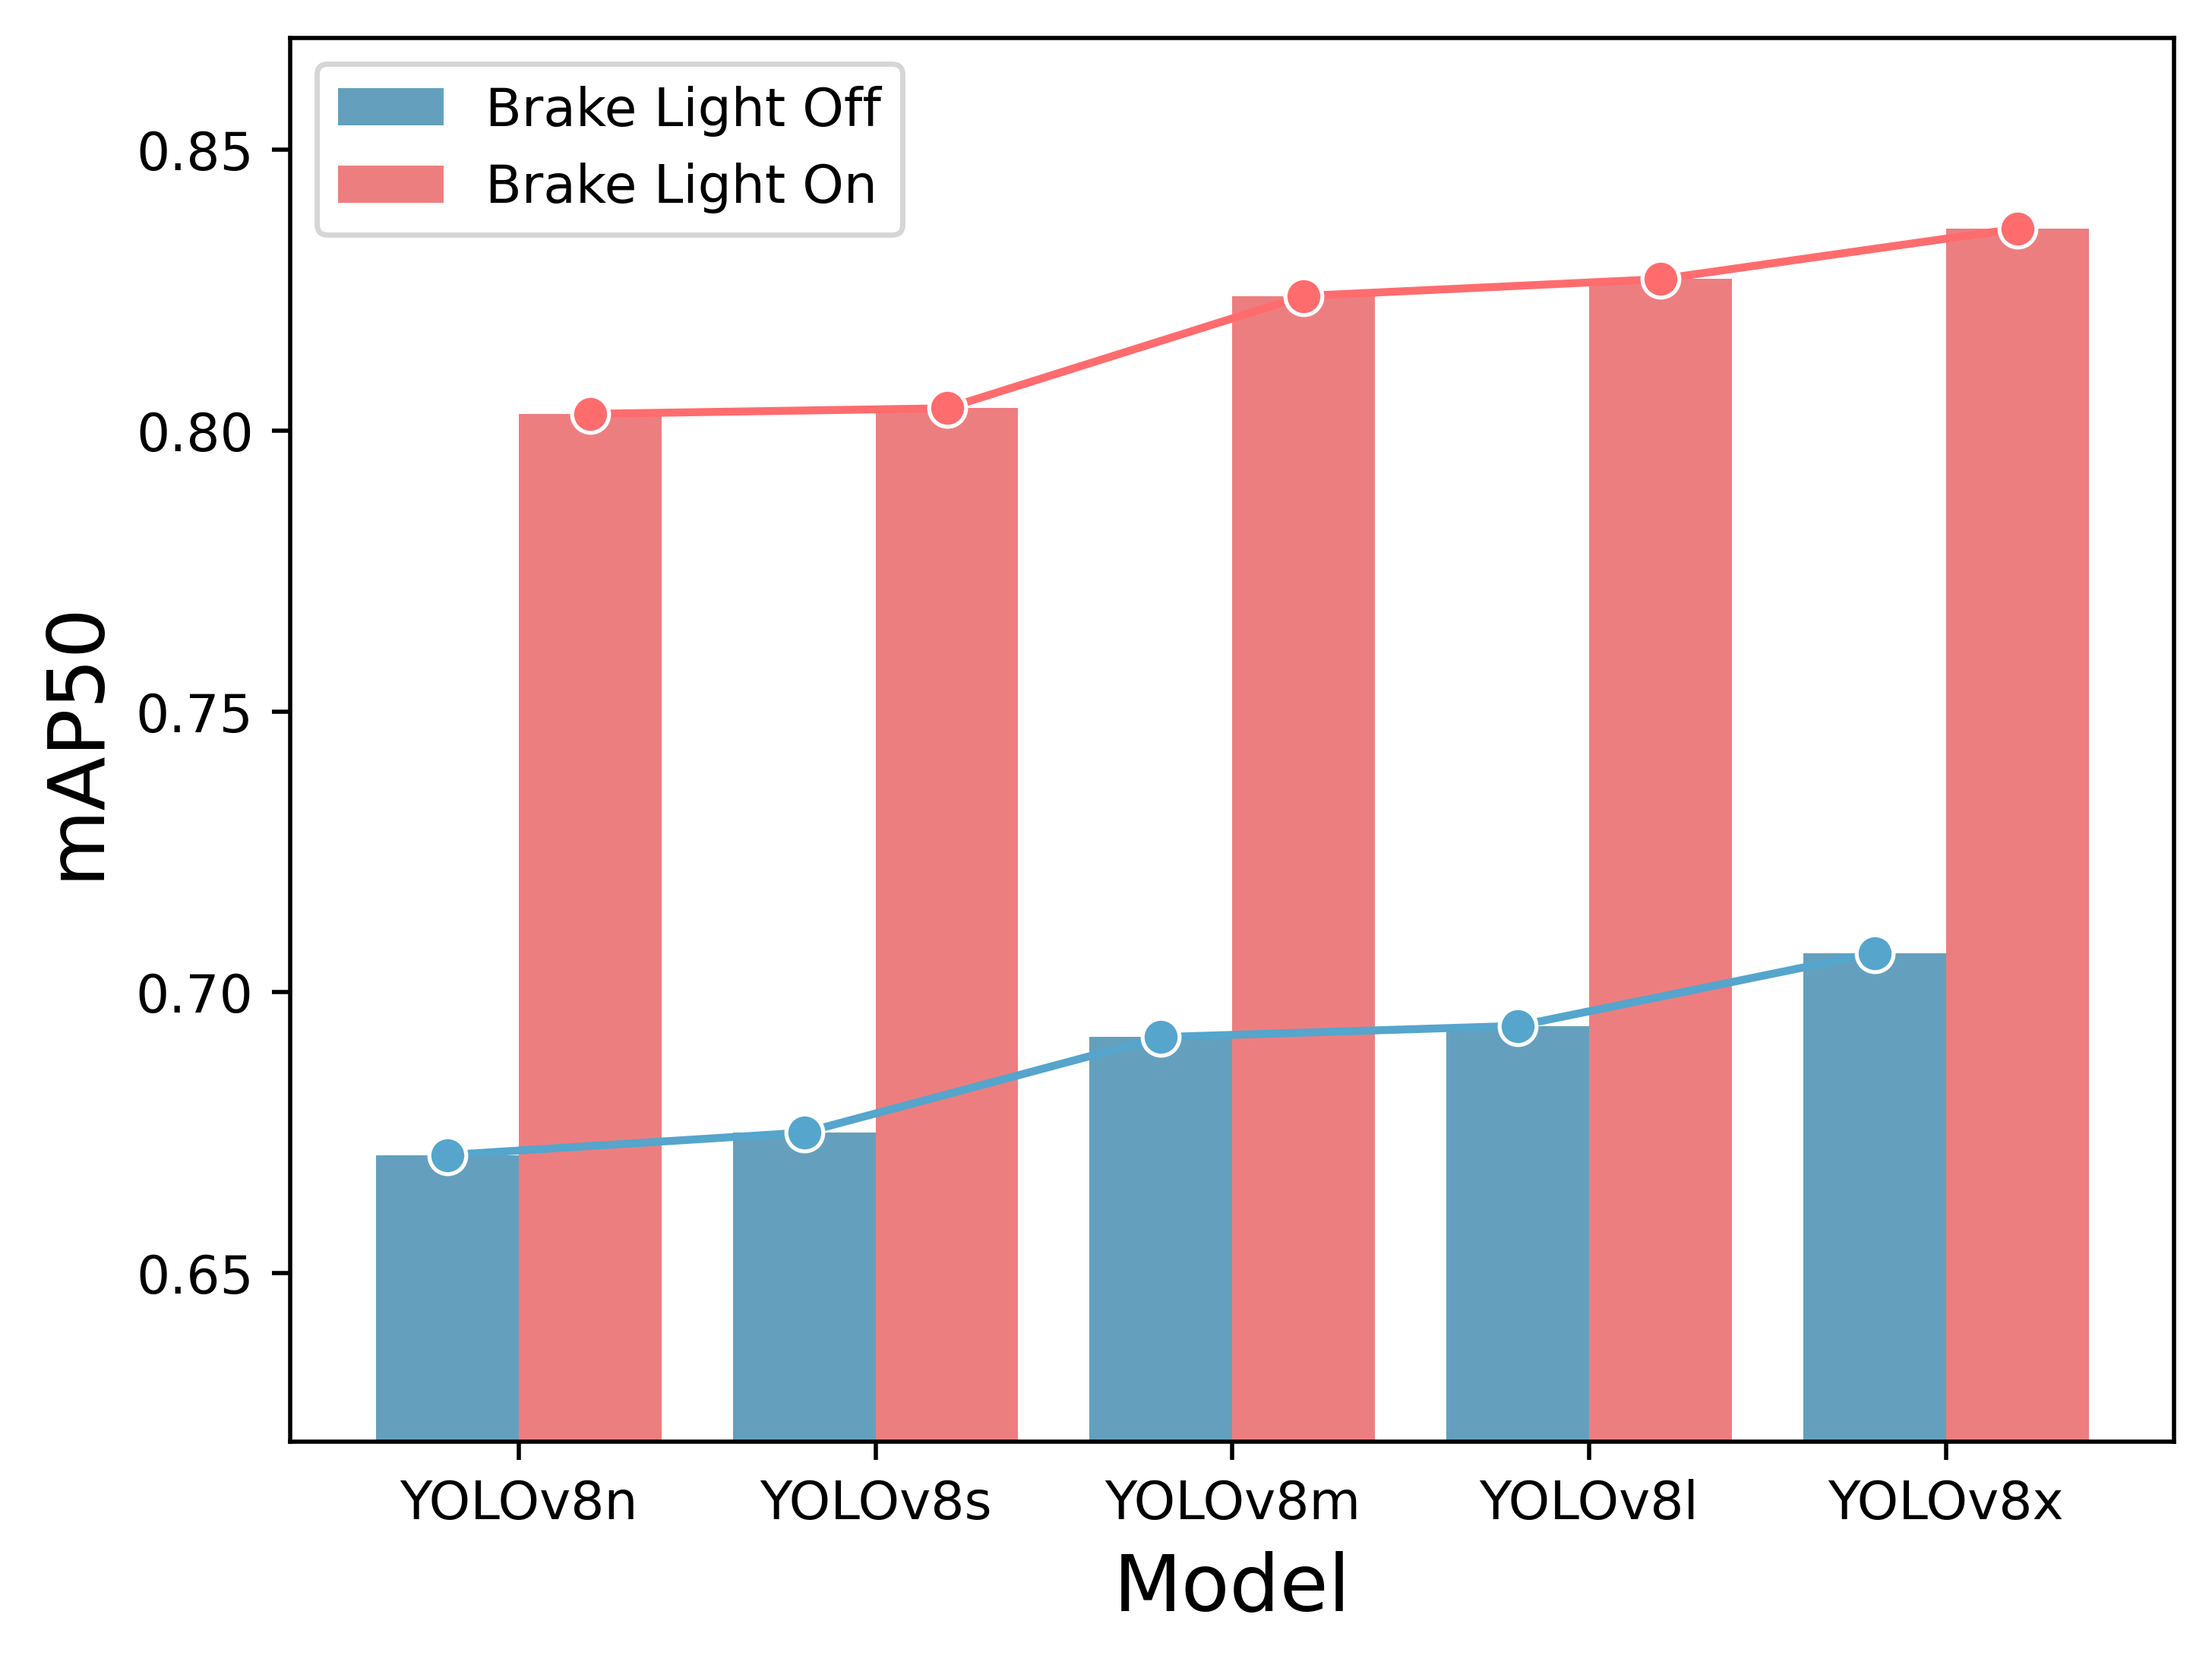
\includegraphics[height=5cm]{fig/bar_night_map50.png} }}%
    \hfill
    \subfloat[mAP50-95 on the Day testset]{{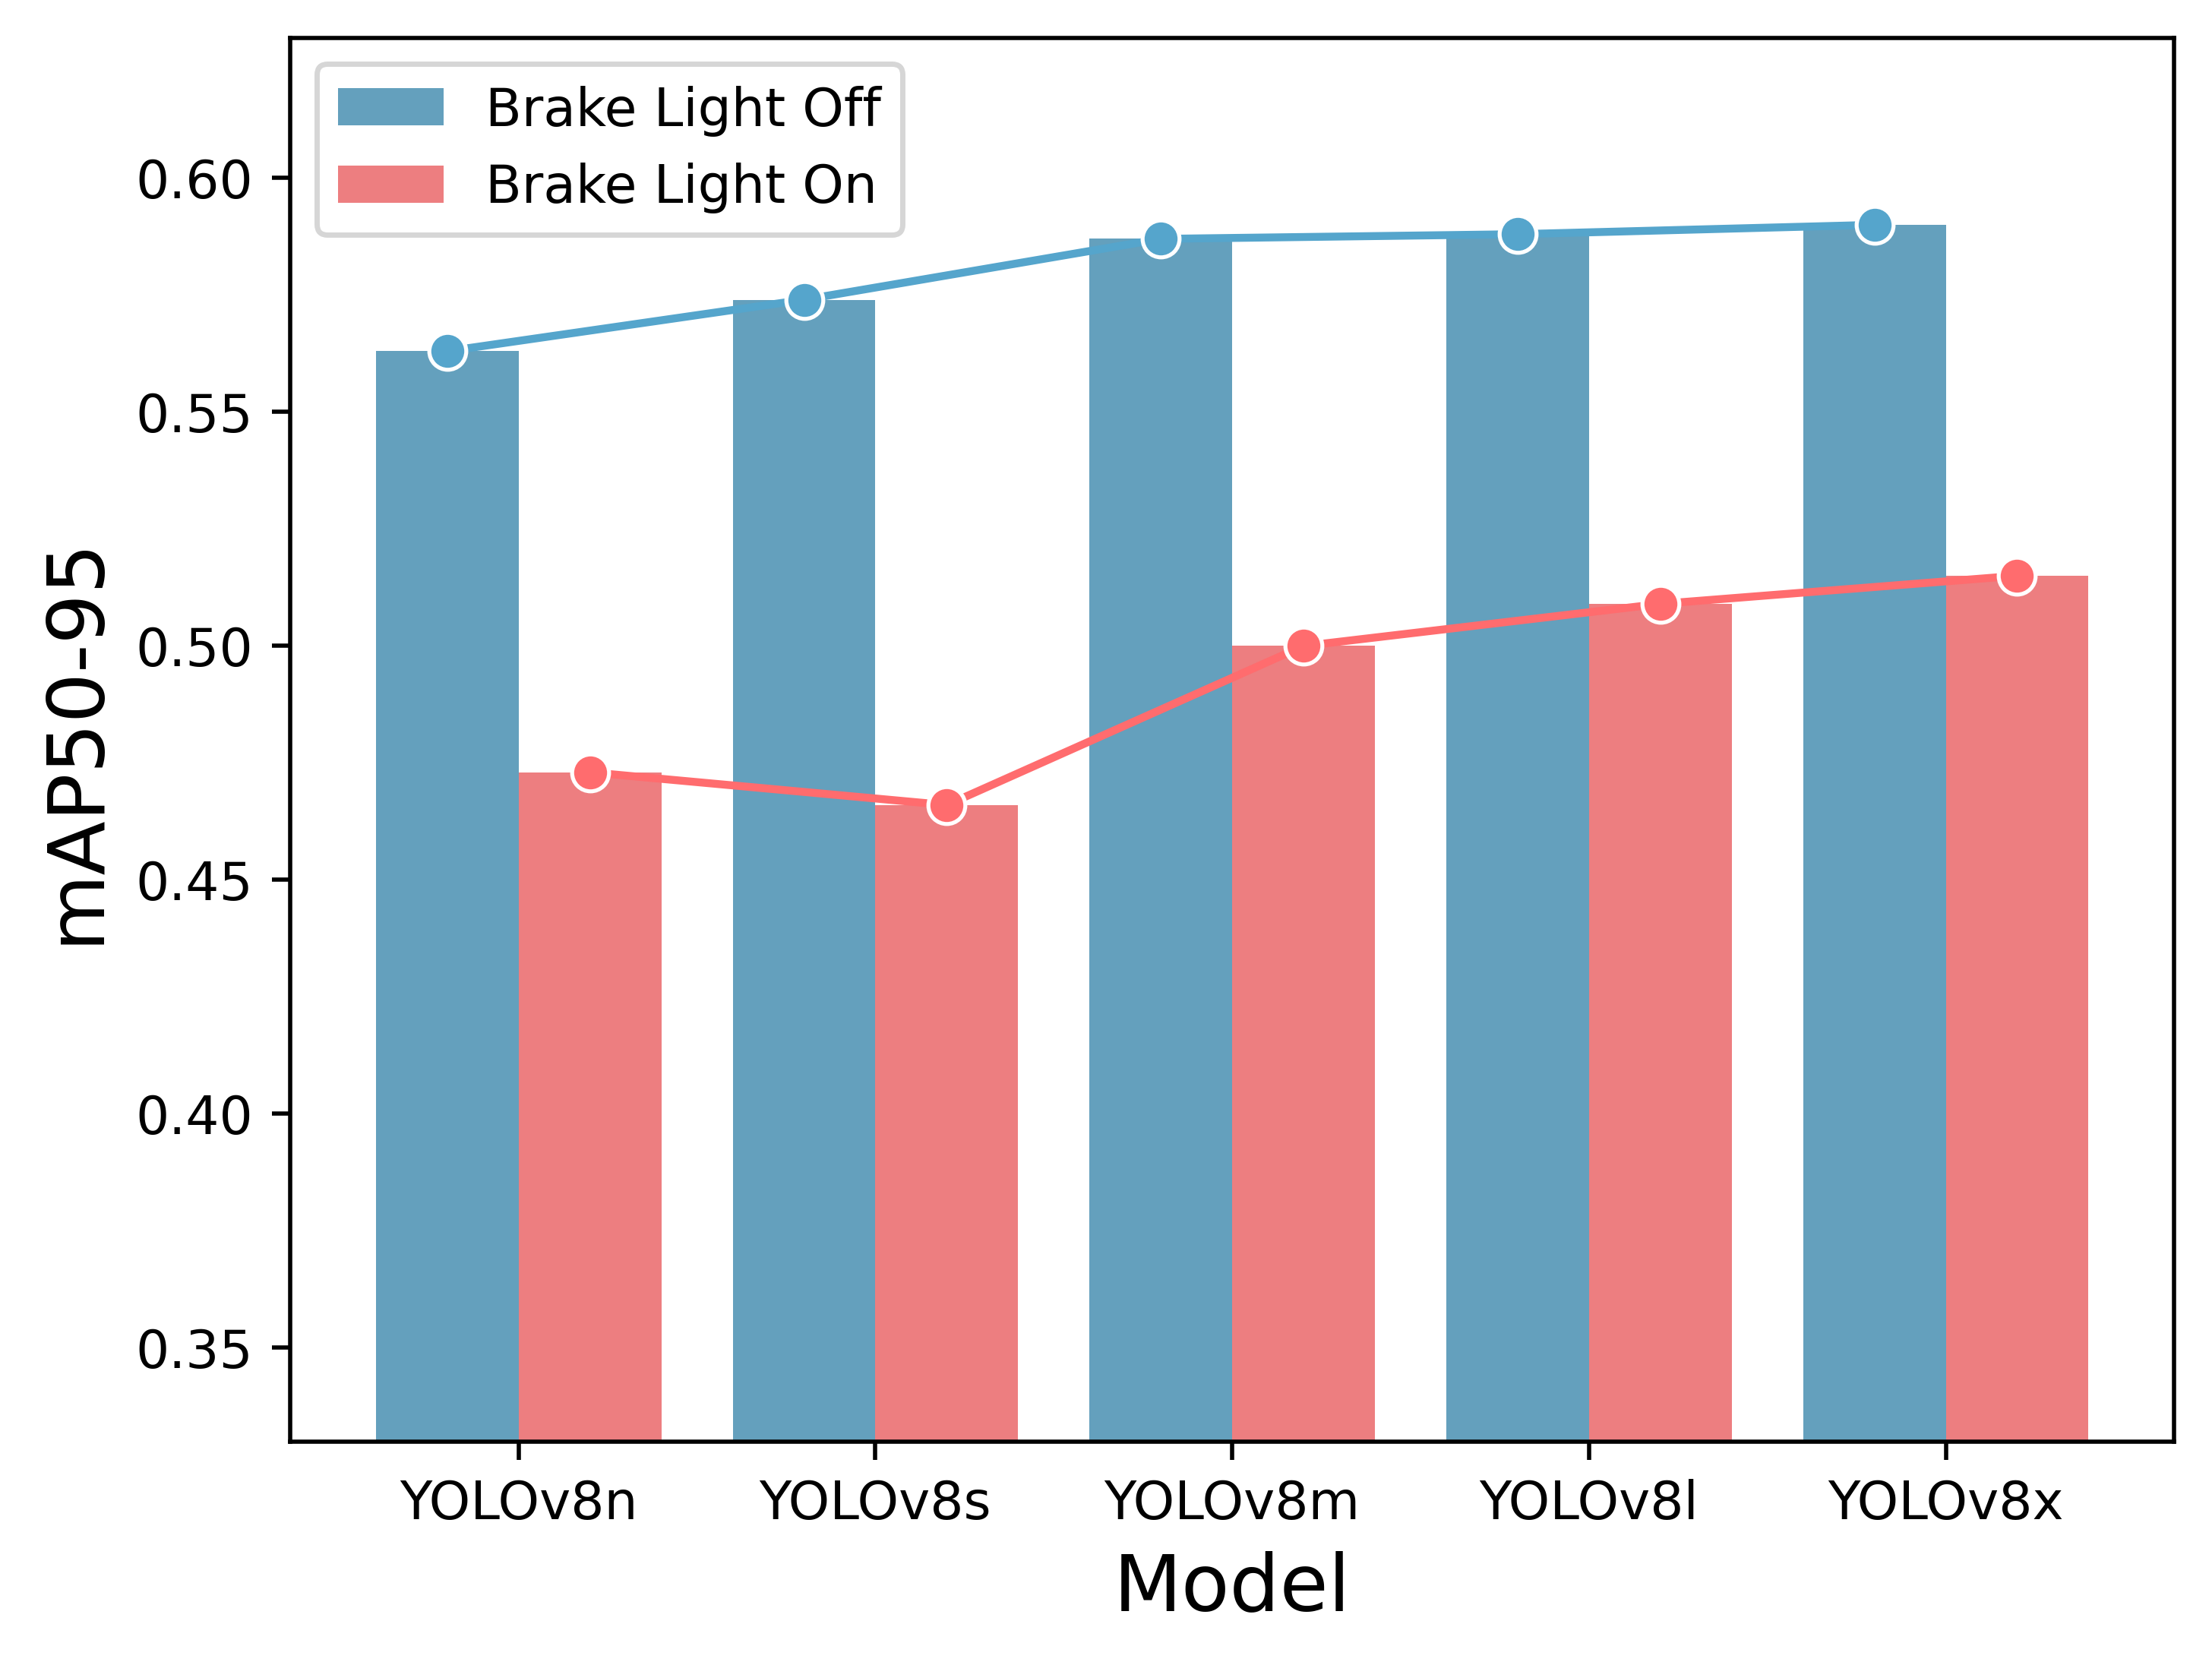
\includegraphics[height=5cm]{fig/bar_day_map50-95.png} }}%
    \subfloat[mAP50-95 on the Night testset]{{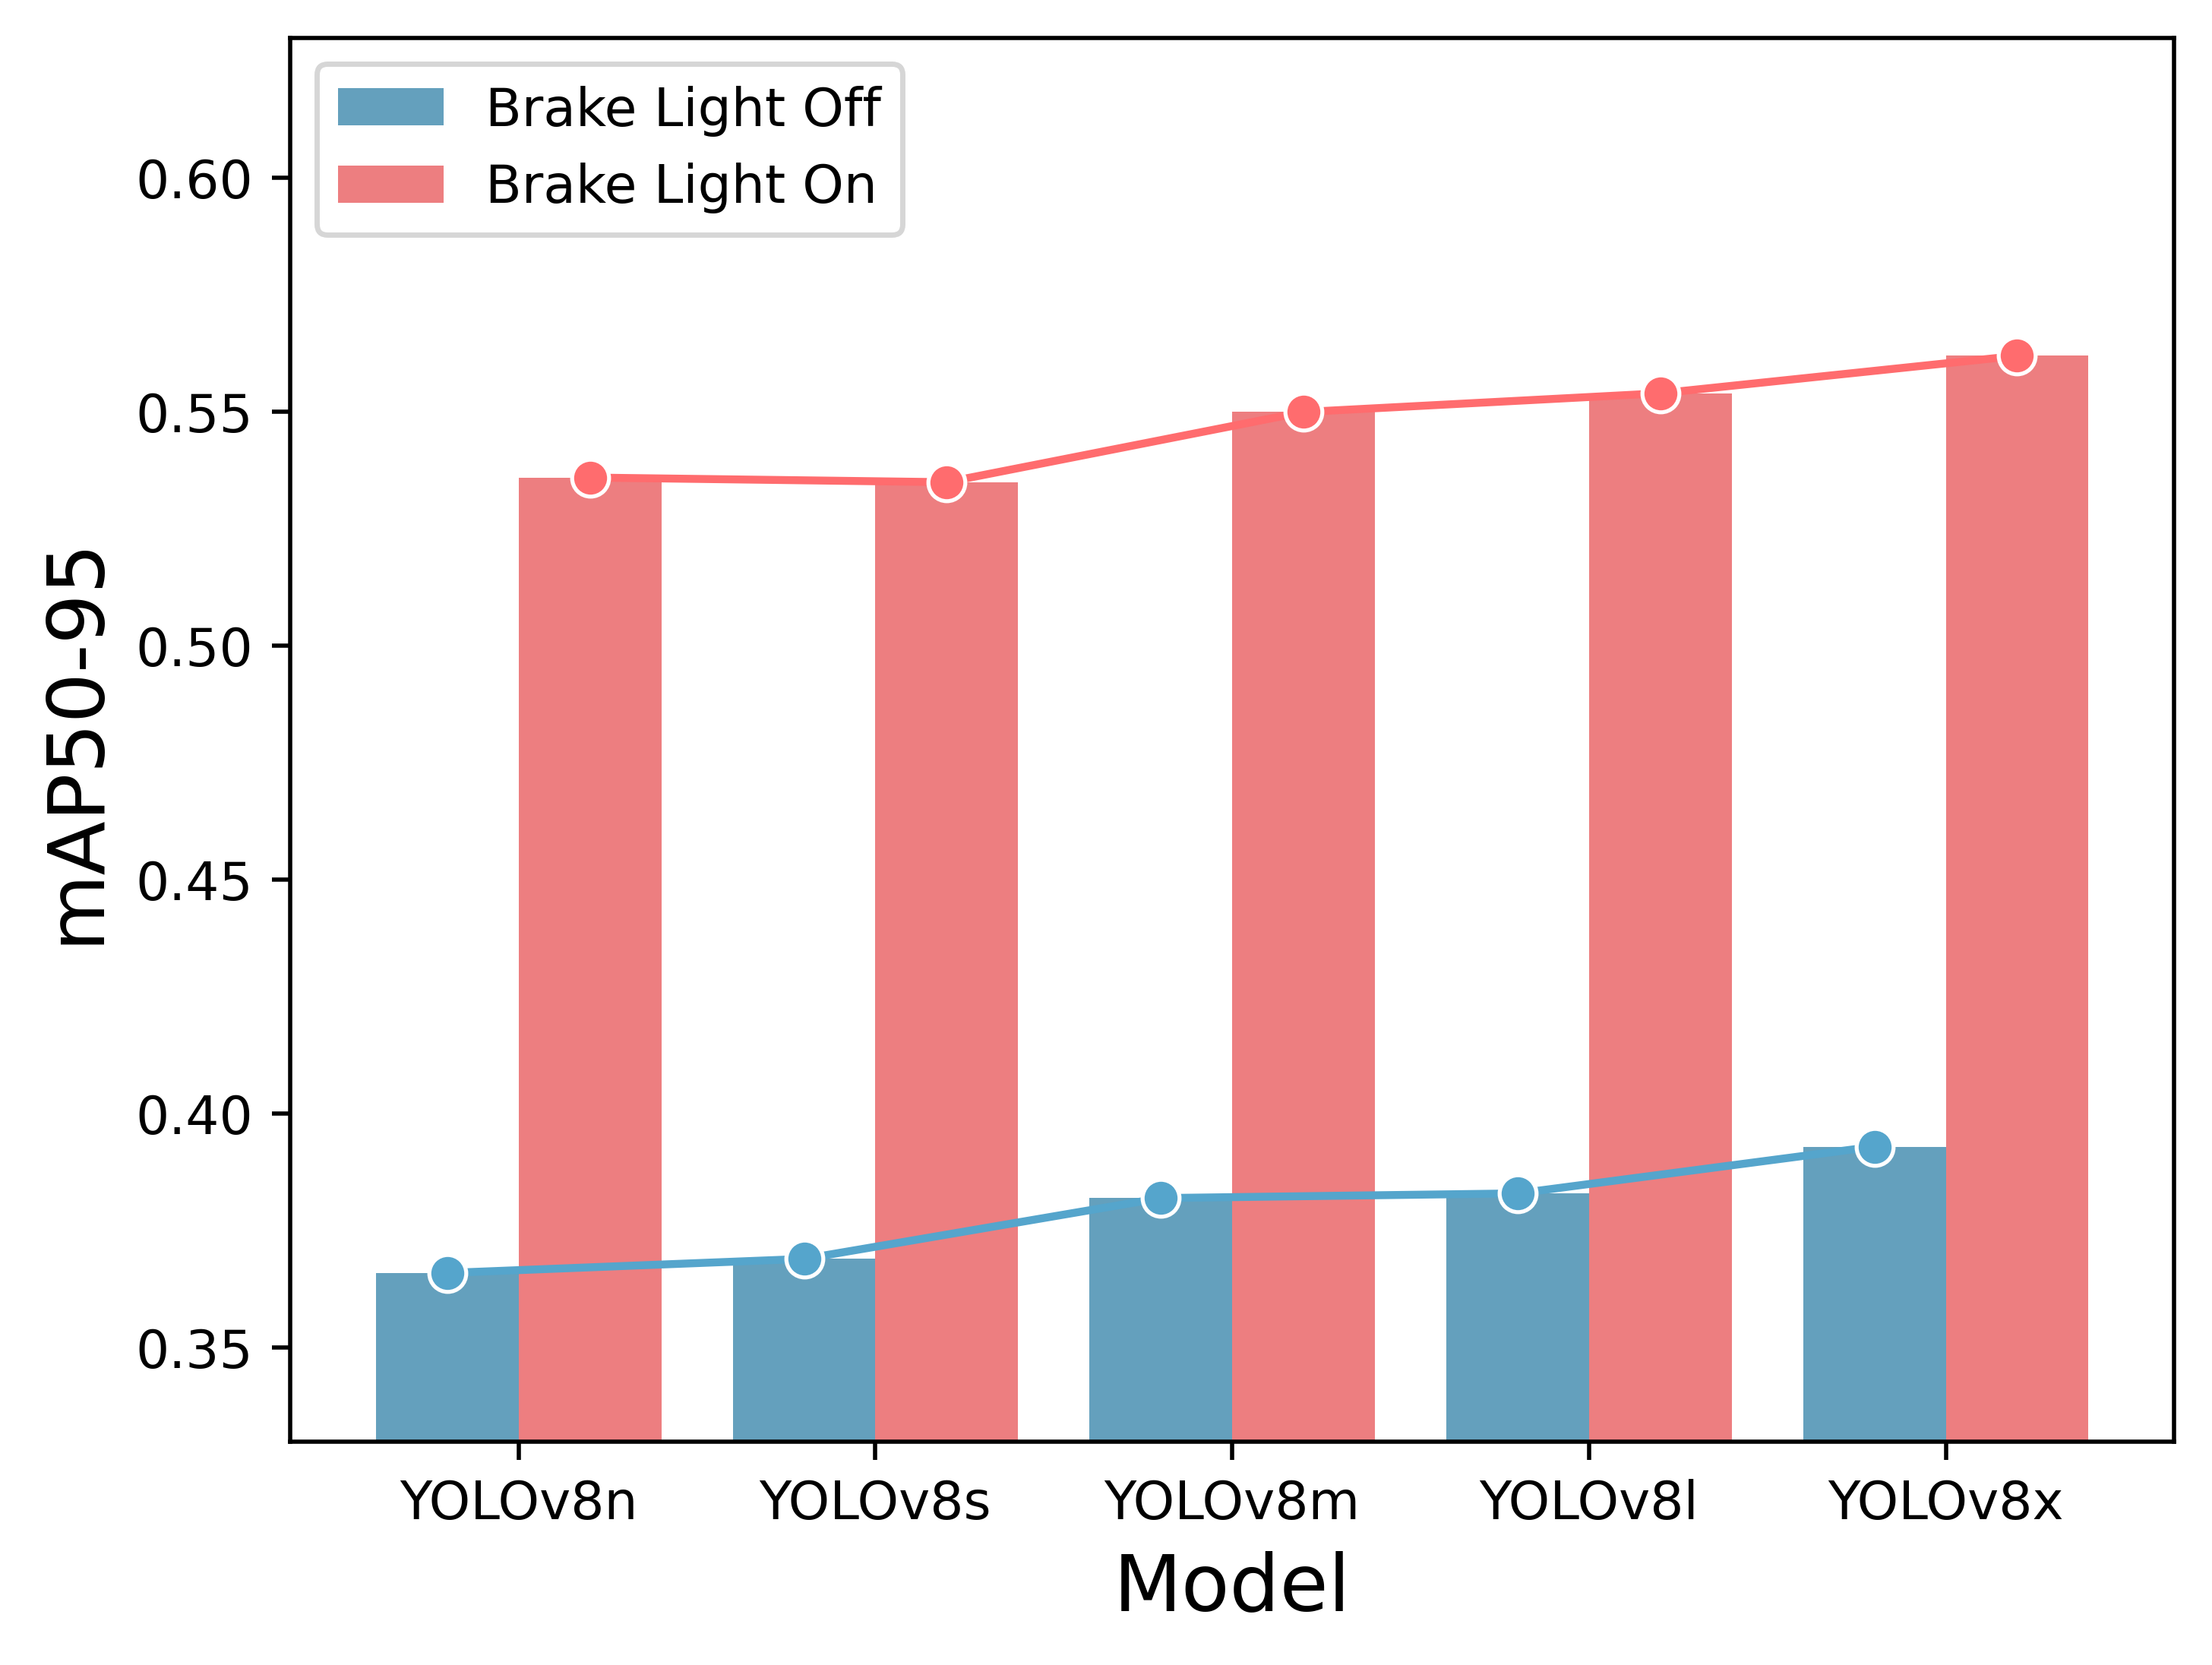
\includegraphics[height=5cm]{fig/bar_night_map50-95.png} }}%

\caption{Detection performance comparison for ambient illumination difference. The y-axis and x-axis represent the detection accuracy and lists the YOLOv8 models, respectively. Each model is depicted with two bars, showcasing the detection performance for brake light off and brake light on classes. Each line plots highlights the difference in detection performance by models for each class.}
\label{fig:dayNnight}%
\end{figure}

Figure \ref{fig:dayNnight} presents the detection performance by each class on the Day/Night split testset. 
Y-axis of Figure \ref{fig:dayNnight}-(a) and (b) represents mAP50 and y-axis of (c) and (d) represents mAP50-95.
Figure \ref{fig:dayNnight}-(a) and (c) shows the performance on the day testset and (b) and (d) shows the performance on the night testset.
On the day testset, brake light off detection performance is better than on detection.
On the night testset, brake light on detection performance is superior to off detection.
The brake light off class, which had been well detected in an environment with high ambient light, deteriorated detection performance as the ambient light decreases.
Conversely, the brake light on class, which had showed relatively low detection performance in an environment with high ambient light, showed high detection performance when the ambient light is low.
The difference in performance due to the difference in ambient illumination is much larger in the brake light off class.
Detailed detection performance comparison for ambient illumination difference for each model and class is described in Table \ref{tab:dayNnight}.


\begin{table}[!b]
    \caption{Results of comparison for ambient illumination difference}
    \label{tab:dayNnight}
    % \resizebox{\textwidth}{!}{%
    \begin{tabular}{llcccc}
    \toprule
    \multicolumn{1}{c}{\multirow{2}{*}{Model}} & \multicolumn{1}{c}{\multirow{2}{*}{Class}} & \multicolumn{2}{c}{mAP50}                           & \multicolumn{2}{c}{mAP50-95}                        \\
    \multicolumn{1}{c}{}                       & \multicolumn{1}{c}{}                       & \multicolumn{1}{c}{Day} & \multicolumn{1}{c}{Night} & \multicolumn{1}{c}{Day} & \multicolumn{1}{c}{Night} \\
    \midrule
    \multirow{3}{*}{YOLOv8n}                   & Brake Light Off                            & 0.808          & 0.671               & 0.563          & 0.366                     \\
    & Brake Light On                             & 0.699                   & 0.803            & 0.473                   & 0.536            \\
    & \multicolumn{1}{r}{Total}                  & 0.753          & 0.737                     & 0.518          & 0.451                     \\

    \midrule
    \multirow{3}{*}{YOLOv8s}                   & Brake Light Off                            & 0.821          & 0.675                     & 0.574          & 0.369                     \\
    & Brake Light On                             & 0.692                   & 0.804            & 0.466                   & 0.535            \\
    & \multicolumn{1}{r}{Total}                  & 0.757          & 0.739                     & 0.520          & 0.452                     \\

    \midrule
    \multirow{3}{*}{YOLOv8m}                   & Brake Light Off                            & 0.822          & 0.692                     & 0.587          & 0.382                     \\
    & Brake Light On                             & 0.729                   & 0.824            & 0.500                   & 0.550            \\
    & \multicolumn{1}{r}{Total}                  & 0.776                   & 0.758                     & 0.544          & 0.466                     \\

    \midrule
    \multirow{3}{*}{YOLOv8l}                   & Brake Light Off                            & 0.821          & 0.694                     & 0.588          & 0.383                     \\
                                           & Brake Light On                             & 0.733                   & 0.827            & 0.509                   & 0.554            \\
                                           & \multicolumn{1}{r}{Total}                  & 0.777          & 0.761                     & 0.549          & 0.468                    \\
    \midrule
    \multirow{3}{*}{YOLOv8x}                   & Brake Light Off                            & 0.825          & 0.707                     & 0.590          & 0.393                     \\
                                           & Brake Light On                             & 0.740                   & 0.836            & 0.515                   & 0.562            \\
                                           & \multicolumn{1}{r}{Total}                  & 0.782          & 0.772                     & 0.552          & 0.477                    \\
    \bottomrule
    \end{tabular}%
    % }
\end{table}



According to the detailed analysis, the performance difference due to the difference in ambient illumination can be explained in terms of accuracy.
Firstly, the overall accuracies for driving vehicle detection across all classes are $0.87$ in the day test dataset and $0.89$ in the night testset.
As the ambient illumination decreases, the accuracy for driving vehicle detection slightly increases.
However, the accuracies for the brake light off class decreases to $0.67$ in the day testset and $0.43$ in the night testset, while the accuracies for the brake light on class increases to $0.75$ in the day testset and $0.86$ in the night testset.
As a results of detailed analysis, the cause of the difference in performance due to the difference in ambient illumination is represented by two factors.
Therefore, as the ambient illumination decreases, the overall detection performance for driving vehicles improves, while the detection performance for the brake light off class deteriorates and the performance for the brake light on class improves.
We argue that this phenomenon is influenced by the tail light.
As the ambient illumination decreases, the tail lights of the vehicles are turned on, which enhances the detection performance for driving vehicles.
However, the turned on tail light causes confusion with the turned on brake light, leading to decreases in the detection performance for brake light off.
As a result, the decrease in ambient illumination enhances the detection performance of vehicles with the brake light turned on, while it deteriorates the detection performance of vehicles with the brake light turned off.


\begin{figure}[!b]
    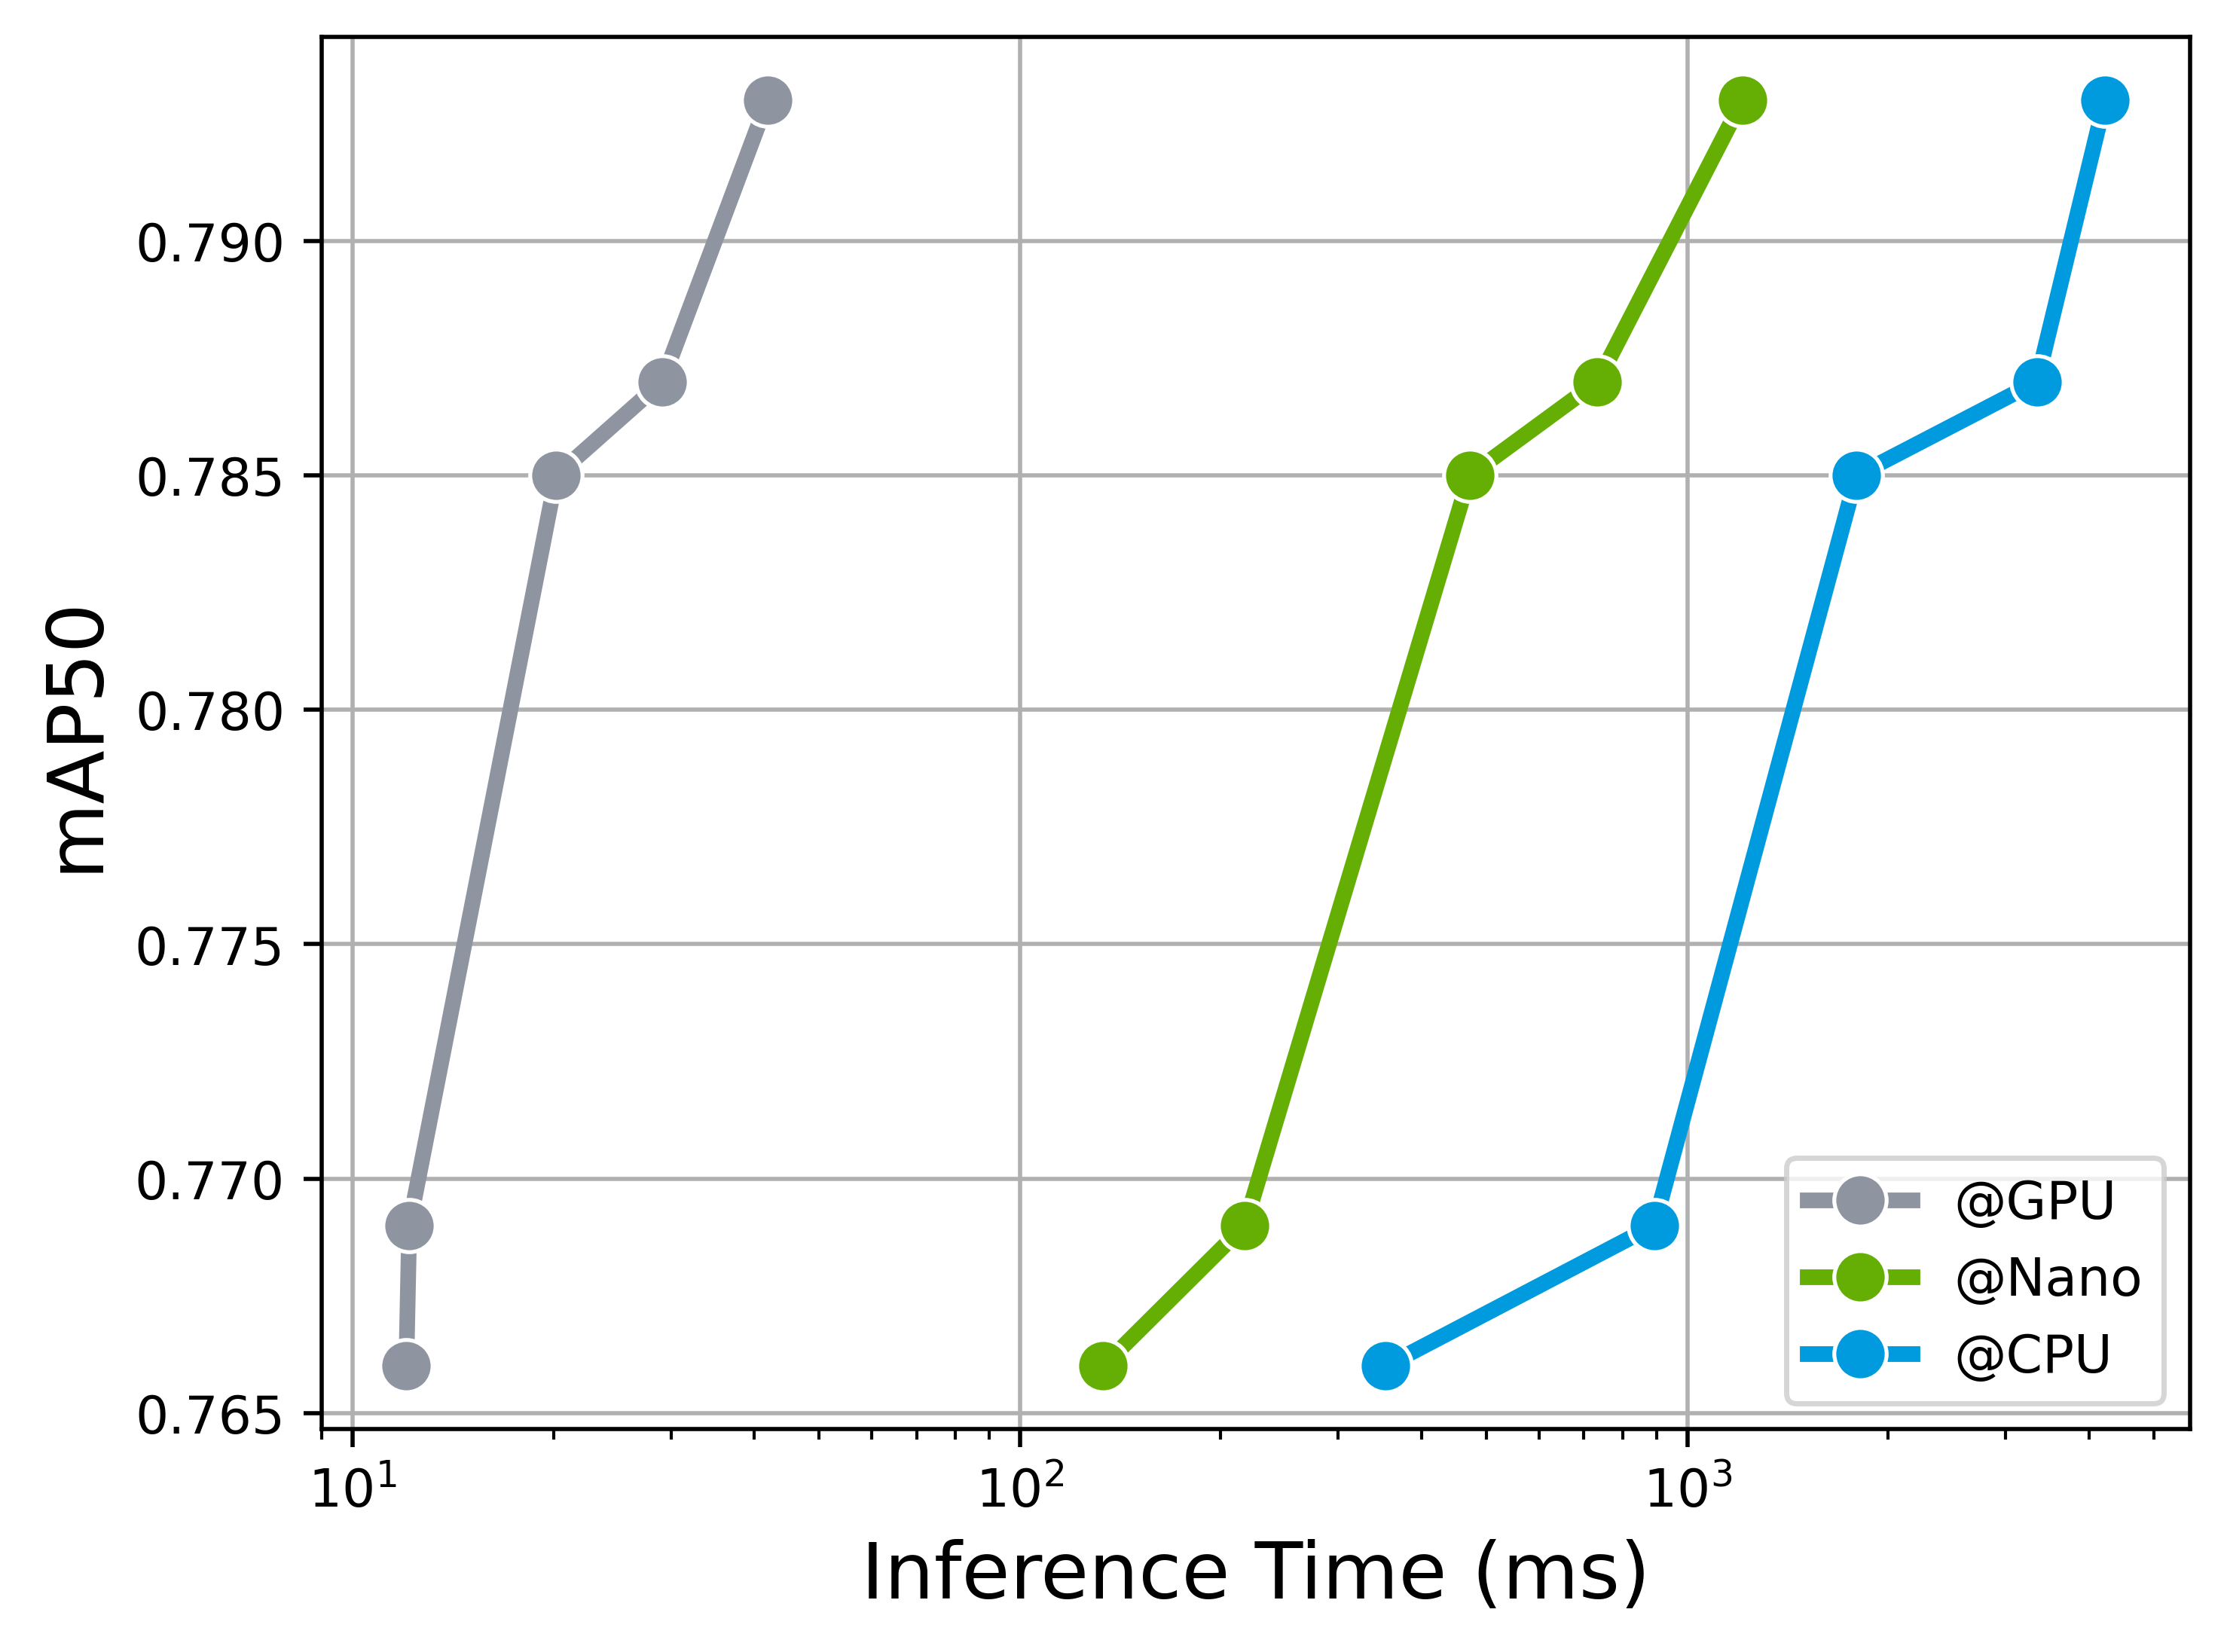
\includegraphics[scale=0.5]{fig/plot_inference_time.png}
    \caption{Trade-off between inference time and detection accuracy in different environments. The x-axis represents the inference time and the y-axis represents the detection accuracy as mAP50. It showcases the trends in inference speed and detection performance for differenct sizes of YOLOv8 under different computing environments as follows:"@GPU" refers to Nvidia Tesla T4, "@Nano" refers to Nvidia Jetson Nano, and "@CPU" refers to Intel Xeon processor.}
    \label{fig:inference}
\end{figure}

\begin{table}[!b]
    \caption{Results of comparision for inference time in different environments. All models were inferred by converting to ONNX form, and the different computing environments are as follows:"@GPU" refers to Nvidia Tesla T4, "@Nano" refers to Nvidia Jetson Nano, and "@CPU" refers to Intel Xeon processor.}
    \label{tab:inference}
    \begin{tabular}{lrrr}
    \toprule
    \multicolumn{1}{c}{\multirow{2}{*}{Model}}   & \multicolumn{3}{c}{Inference Time (ms)} \\
                                 & ONNX @GPU & ONNX @Nano & ONNX @CPU \\
    \midrule
    YOLOv8n & 12.04        & 133.30            & 353.13    \\
    YOLOv8s & 12.16        & 217.20            & 891.93    \\
    YOLOv8m & 20.20        & 471.59            & 1792.31   \\
    YOLOv8l & 29.09       & 733.27            & 3340.26   \\
    YOLOv8x & 41.87       & 1208.69           & 4222.87  \\
    \bottomrule
    \end{tabular}%
\end{table}

Given our research objective of real-time detection in driving vehicles, it is essential to conduct experiments not only to achieve accurate detection but also to evaluate the inference time. Particularly, verification on edge devices with limited computational capacity and power consumption is crucial. To validate real-time inference on edge devices, we utilized Nvidia's Jetson Nano device.
We converted the trained model to the Open Neural Network Exchange (ONNX) format and measured the inference time on the Jetson Nano Device.
ONNX is an open format that allows sharing and interoperability of neural network models, serving as a standardized format for mutual conversion between various frameworks.
The inference times ranged from $133.30$ ms to $733.27$ ms, depending on the model size. 
Considering that brake light status detection is a perception algorithm aimed at improving the ride comfort of ADAS or autonomous driving systems, the achieved inference time of 133.30ms with the smallest model, the YOLOv8n, can be deemed sufficiently real-time.
The trade-off performance between inference time and detection accuracy is shown in Figure \ref{fig:inference}.
To provide an intuitive performance comparison, we included the performance on not only the Jetson Nano but also on CPU and GPU.
The CPU device used was Intel Xeon 2.20GHz, and the GPU device used was Nvidia Tesla T4.
Detailed values are described in Table \ref{tab:inference}.



